\documentclass[a4paper, twoside]{report}

\usepackage[english]{babel}
\usepackage[utf8]{inputenc}
\usepackage{csquotes}
\usepackage[T1]{fontenc}
\usepackage{listings}
\usepackage{hyperref}
\hypersetup{colorlinks=false}
\usepackage{lscape}
\usepackage{amsmath}
\usepackage{graphicx}
\usepackage[colorinlistoftodos]{todonotes}
\usepackage[ruled, vlined]{algorithm2e}
\usepackage{verbatim}
\usepackage{subcaption}
\usepackage{float}
\usepackage{tikz}
%\usepackage{algpseudocode}
\usepackage{tabularx}
%\usepackage{multirow}
\usepackage{makecell}
\usepackage{biblatex}
\usepackage{enumitem}
\usepackage{pgfgantt}
\usepackage{rotating}
\usepackage{amssymb}
\usepackage{cleveref}
\usepackage{rotating}
\usepackage{threeparttable}
\usepackage{appendix}
\usepackage{xcolor}
\usepackage{bluespec}
\usepackage{minted}
\usepackage{tcolorbox}
\usepackage{etoolbox}
\BeforeBeginEnvironment{minted}{\begin{tcolorbox}}%
\AfterEndEnvironment{minted}{\end{tcolorbox}}%
\usepackage[compatibility=false]{caption}
\usepackage{dirtree}
\usepackage[nounderscore]{syntax}


\usepackage{array}

\newenvironment{conditions}
  {\par\vspace{\abovedisplayskip}\noindent\begin{tabular}{>{$}l<{$} @{${}={}$} l}}
  {\end{tabular}\par\vspace{\belowdisplayskip}}


\addbibresource{main.bib}
\def\checkmark{\tikz\fill[scale=0.4](0,.35) -- (.25,0) -- (1,.7) -- (.25,.15) -- cycle;}

\usemintedstyle{perldoc}

\lstdefinestyle{verilog-style}
{
    language=Verilog,
    basicstyle=\small\ttfamily,
    keywordstyle=\color{vblue},
    identifierstyle=\color{black},
    commentstyle=\color{vgreen},
    numbers=left,
    numberstyle=\tiny\color{black},
    numbersep=10pt,
    tabsize=8,
    moredelim=*[s][\colorIndex]{[}{]},
    literate=*{:}{:}1
}

\makeatletter
\newcommand*\@lbracket{[}
\newcommand*\@rbracket{]}
\newcommand*\@colon{:}
\newcommand*\colorIndex{%
    \edef\@temp{\the\lst@token}%
    \ifx\@temp\@lbracket \color{black}%
    \else\ifx\@temp\@rbracket \color{black}%
    \else\ifx\@temp\@colon \color{black}%
    \else \color{vorange}%
    \fi\fi\fi
}
\makeatother


%% Sets page size and margins
\usepackage[a4paper,top=3cm,bottom=2cm,left=3cm,right=3cm,marginparwidth=2cm]{geometry}

\begin{document}
    \begin{titlepage}
        % \newgeometry{top=25mm,bottom=25mm,left=38mm,right=32mm}
        \setlength{\parindent}{0pt}
        \setlength{\parskip}{0pt}
        % \fontfamily{phv}\selectfont

        {
                        \Large
                        \raggedright
                        Imperial College London\\[17pt]
                        Department of Electrical and Electronic Engineering\\[17pt]
                        Final Year Project Report 2014\\[17pt]

        }

        \rule{\columnwidth}{3pt}
        \vfill
        \centering
        \vfill
        \setlength{\tabcolsep}{0pt}

        \begin{tabular}{p{40mm}p{\dimexpr\columnwidth-40mm}}
                        Project Title: & \textbf{High-level Synthesis for multi-FPGA systems} \\[12pt]
                        Student: & \textbf{Naim Govani} \\[12pt]
                        CID: & \textbf{01371045} \\[12pt]
                        Course: & \textbf{EIE4} \\[12pt]
                        Project Supervisor: & \textbf{Dr David Thomas} \\[12pt]
                        Second Marker: & \textbf{Dr John Wickerson} \\
        \end{tabular}
    \end{titlepage}

    \begin{center}
        \textbf{\huge Final Report Plagiarism Statement }
    \end{center}

    \noindent I affirm that I have submitted, or will submit, an electronic copy of my final year project report to the provided EEE link. \\ \\
    I affirm that I have provided explicit references for all the material in my Final Report that is not authored by me, but is represented as my own work.
    \newpage
    
    \setlength{\parskip}{4pt}
    \setlength{\parindent}{4pt}

    \begin{abstract}
    Multi-FPGA systems have usually only been accessible to individuals who are already proficient in the use of FPGA tools and hardware design. This fact seems unfortunate since the necessity for latency-critical systems has increased in the last few years with larger datasets needing to be processed. Multi-FPGA systems offer the parallelism needed to compute these tasks in a reasonable time, however their accessibility fall short of their demand. SystemNaim is tool which aims to explore the possibility of making multi-FPGA systems more accessible to those not proficient in hardware design. The tool allows the user to program a system in the C90 language, and then through the use of function calls, split the resulting system across multiple FPGAs.
    
    In this paper, we will go through the motivation, design methodology, and implementation of SystemNaim and then evaluate, using both qualitative and quantitative methods, whether it achieves it's intended purpose. We will prove that while the tool creates less optimal hardware than a dedicated system, the time saved by using the tool, potentially weeks, can allow for much more experimentation and larger systems to be implemented in reasonable times. We will also show that programs which have an affinity for parallel execution are most the most appropriate to be implemented using SystemNaim, with examples showing up to a 42\% reduction in latency when run on a multi-FPGA system.
\end{abstract}

    \tableofcontents    
    % if you are adding a new chapter, create a new folder in the root directory of the project
    % it should begin with a two digit number, followed by an underscore and the name of the section.
    % This keeps the order of the sections in the side view in keeping with the order of the document.


    
    \chapter{Project Introduction}

\begin{itemize}
    \item Introduce aim of project: To prove it is possible to create a multi-fpga system through an HLS Tool.
    \item There are benefits to completing the aim above and that will be explored later
    \item Maybe talk about the fact that the HLS part isn't that important to the investigation. Likely to introduce the concept and then elaborate further in the design section.
    \item Also talk about what contributions we are aiming to achieve:
    \item Split below into two parts, one is project aims/objetives (questions) and one into what was actually accomplished and produces
    \begin{itemize}
        \item HLS tools make it easier for users to create dedicated hardware.
        \item It is possible to automate the process of creating a multi-FPGA system and integrate it into a HLS tool
        \item This automated process can provide a performance boost and does not add too much of an overhead.
        \item In summary, we can make it easier for people to create a multi-FPGA system, thus allowing people who could benefit from such a thing(Researches, ...?), to do so without requiring an exorbitant amount of extra man-power.
        \item The hls tool is a platform for Researches
        \item the interconnect
    \end{itemize}
\end{itemize}
    \chapter{Background}
\label{chap:Background}

\section{Introduction}

The field of multi-FPGAs has been heavily researched however there are few papers interested in utilising HLS to streamline the process of implementing a multi-FPGA. \cite{564741} and \cite{707888} are examples of papers which do concern themselves with these topics but both were written over twenty years ago.

Therefore, it is of interest to this project to do a review of the most up to date research in fields surrounding and including its scope. This chapter will go through five different topics:

\begin{itemize}
    \item Related works.
    \item HLS tools and their optimisations.
    \item FPGA-to-FPGA communication protocols.
    \item Multi-FPGA Logic Partitioning.
    \item RPC systems.
\end{itemize}

Thus, hopefully, giving the reader a better overview of what is possible if this project were to reach its full potential.

\section{Related Work}
\label{sec:related_work}

As previously mentioned, \cite{564741} and \cite{707888} are papers which have already attempted to solve the issues raised by this project. The solution in the former uses the GNU C++ compiler as well as a method of describing the algorithm as a set of difference equations. One point the authors explicitly state is that they utilise C++'s operator overloading feature in order to map software operations to specific hardware modules. Nonetheless, once the circuit has been generated, it is then automatically partitioned using a method based on Fiducia-Mattheyses bi-partitioning heuristic \cite{1585498} with the goal of this stage to maximise logic utilisation in each FPGA as well as minimising IO consumption.

The method by which the FPGAs communicated with each other is not discussed in the paper, all that is mentioned is the method used for partitioning. There is, however, mention of a host CPU, and it may be reasonable to assume that this CPU acts as a master for all FPGAs meaning there is no direct communication between FPGAs.

The latter paper, \cite{707888}, opts to place a psuedo-processor on each FPGA within the topology and then have a top-level controller supply each FPGA with the instructions it is meant to execute. The HLS aspect then merely needs to convert the supplied source code into a list of instruction which is the intended use of standard compilers. The motivation for this approach was to make multi-FPGA systems more accessible to software developers, which is its main target demographic. Alongside this, the paper also presents how it uses a 4 dimensional space, with one dimension being each FPGA system, to optimise the datapath of the system. This then supposedly creates a control path where the FPGAs are used in parallel wherever possible.

\section{HLS Tools \& Optimisations}
\label{sec:bg:hls}

\subsection{Introduction}

Different HLS tools have vastly different implementations \cite{7368920} and many of them, especially commercial tools, do not reveal their methodologies. LegUp\cite{legup} for example, compiles the input source code using the LLVM compiler and then profiles it on a modified MIPS CPU emulator in order identify which parts of the code would benefit from hardware acceleration. It then synthesises those specific parts to dedicated hardware, while the rest of the code is run using a MIPS CPU programmed onto the FPGA.

Vivado HLS, on the other hand, makes no attempt to suggest to the user where acceleration is possible. Rather, it merely gives you tools known as PRAGMAS, found in \cite{vivado-optmisation-manual}, to help the compiler better understand how to convert the C code to hardware. The output is then a set Verilog files the user can implement as they see fit, though it is recommended to use the Vivado Design Suite \cite{vivado-design-suite-manual} as part of the development cycle. As of now, Vivado has not revealed how they go from C to Verilog.

A third contender is Bambu~\cite{6645550}, which leverages the GCC IR in order to optimise the resulting hardware and focuses mainly on memory intensive programs. In short, each implementation has its own intended purpose and thus excels in a specific area, but the fact that there are many implementations indicate that this field has much room from improvement and is actively under development.

\subsection{Input Language}

For the most part, HLS tools tend be based around compiling a subset of C or C++ to Verilog \cite{7368920}, however, there is an argument to be made that functional programming languages have a certain affinity towards hardware development. \cite{bjesse1998lava} presents an early form of the idea, Lava, which takes Haskell as input and produces circuit specifications. The tool was built in the early days of HDLs, and thus was intended to be a competitor rather than a part of the tool chain. More modern approaches such as \cite{hardcaml} are libraries for existing languages and instead produce Verilog or SystemVerilog which can be later synthesised by the appropriate tools. But why bother with straying so far from the norm. In \cite{7331371}, it is suggested that the firm mathematical founding in which functional languages are based can assist in verifying hardware designs as well as offering benefits such as recursive functions and type inference. While the author in \cite{Edwards2019FHWP}, suggests that the functional paradigm can allow for a greater exploitation of parallelism, one of the driving reason to using FPGAs. 

Evidently, the field of research in using functional languages is of interest to quite a few individuals. \cite{7723553} lists a few papers in its introduction whilst also contributing to the field itself, but it has yet to be seen whether Functional HLS will overtake standard C-based HLS anytime soon.

\subsection{Loop Pipelining}

One of the major benefits of running a system on an FPGA is its ability to perform computation in parallel. Loop pipelining is a perfect example of this, where a HLS tool will take a for loop or while loop written in the source code and run segments of it concurrently in order to reach a low initiation interval(II). Page 120 of \cite{vivado-optmisation-manual} and page 11 of \cite{intel-hls-manual} show how the two leading HLS tools, Vivado HLS and Intel High Level Synthesis Compiler, implement pipelining respectively. The II is a measure of how many a new iteration of the loop can start and a lower value, ideally one, means that the section of code containing the loop will be computed faster. 

There are issues, however, with attempting to reach an $II = 1$. \cite{7544750} explores how memory dependencies, two parts of a loop accessing the same memory resources, can cause increases in II due to the HLS compiler not being able to find a way to resolve these dependencies. Instead, it proposes the idea of splitting loops in order to reach an II of 1 on each of these sub-loops and then to pipe the data from one sub-loop to the next. Another approach shown in \cite{7160061} opts to implement parametric hardware to resolve similar dependencies. 

In summary, for simple programs with static loop behaviour the loop pipelining strategies found in commercial tools is very effective and likely the most important optimisation. However, when the behaviour becomes uncertain more effort is required on the user's side to help the compiler reach lower II's.

\subsection{Data Streaming}

In order to process data in parallel on an FPGA the data must first be available to the device or module doing the processing, an obvious point but one that must be considered for any HLS system. In general, there are two approaches to solve the problem of ensuring data availability, the first is atomic transactions while the second is data streaming/dataflow. Say that we have two modules, $A$ and $B$ which are connected such that the output of $A$, which is an array, is the input of $B$. Let us also say that both modules iterate over an array doing some processing, i.e. multiplying the elements by 2 or adding 5, on said array. In an atomic system we would first let $A$ iterate over the entire array and then pass the array to $B$ and allow it to compute its function. 

In this case, even though the modules themselves may be pipelined there isn't much parallelism being exploited on the module level. $B$ is sitting idle for the entire time $A$ is operating and vice-versa. The solution to this is dataflow, which is where every time $A$ completes an iteration it then passes that data to $B$ allowing to start its computation. This results in both modules being utilised at the same time and reduces the overall latency of the system. Section 3.3 of \cite{9264692} explores further, why a user might opt for this method and the considerations they must take if they choose to do so. 

In relation to HLS tools, this optimisation is pivotal to achieving high throughput in any system that operators on large amount of data. Pages 20-24, 95-97 and 126-128 of \cite{vivado-optmisation-manual} show how Vivado HLS allows its users to access such functionality.


\section{FPGA-to-FPGA Communication}
\label{sec:bg:comm}

\subsection{Communication Medium}

One of the major considerations that must be made when deciding the structure of a multi-FPGA system is the communication medium between the FPGAs. Many options are possible, \cite{10.1145/3358192} utilises SFP+ connections whilst \cite{10.1145/3337821.3337846} connects the board using a PCI-E interface. Both examples require ports to be connected to FPGA I/O pins and are usually approaches that are, usually, only used when working development boards. If, one only has access to the pure FPGA itself, unlikely nowadays, then pin implementations are a much more apt choice. \cite{658564} goes into very fine detail about the necessity of a good pin assignment algorithm to reduce unnecessary resource consumption.

It seems that more modern implementations tend to use a standardised communication medium such as Ethernet, PCI-E or Serial, which makes sense given the large overhead usually required when developing a new communication protocol. \cite{7890234} even explores making the communication medium agnostic to the user application, which allows the user logic to access a single interface which then handles to packaging of data for any medium. For example, one FPGA may only have access to an Ethernet port while another only has an RS232 port, but this system would allow these two FPGA's to transfer data between them.

\subsection{Purpose of the System}

While there are many options for communication mediums available to a designer, one must first question the purpose of the system in order to evaluate the efficacy of a communication method. 

A \textbf{PCI-E} communication medium tends to be chosen when there is a single host communicating with multiple client's such as in \cite{10.1145/3337821.3337846} or \cite{6927459}. PCI-E does not allow for clients to interact directly with each other and instead only allows host-client communication. 

In contrast, \textbf{Ethernet} allows the user to identify each device in their topology with a number (MAC Address) and then lets each device send data to every other device in the network (Section 8 in \cite{6847097}) making it more suited to Peer-2-Peer systems. 

Both have their place in the ecosystem with latest PCI-E generations reaching 128 GB/s \cite{pcie-speed} compared to Ethernet reaching at most 1.25 GB/s \cite{ether-speed}, whilst is Ethernet better suited for more complicated topologies with numerous hosts.

\section{Logic Partitioning}
\label{sec:logic_part}

\subsection{Manual vs. Automatic}

Logic partitioning concerns itself with how a designer split's the computation across the multi-FPGA system. Generally speaking, there are two approaches to this a manual split and an automatic split. A manual split is where the designer is given control of the computation processed on every FPGA, however usual implementations following this methodology tend to be a single design replicated on multiple FPGAs. \cite{10.1145/3020078.3021739, 10.1145/3358192, 10.1145/3337821.3337846} all have one FPGA overlay that supports communication either with a host or other peers and is able to slot into a pre-existing network in a modular fashion. Thus, it would seem that any manual splitting is done with scalability in mind and a repeatable design is used to reduce decrease complexity and development time.

The second approach is an automatic split, and it seems that papers regarding this method tend to concern themselves with more general input than a specific use case. Both papers mentioned in \autoref{sec:related_work} and \cite{soton261305} are examples of this approach. Interestingly, \cite{707888} uses a similar practice to what was described of the manual approach by having a single design, that has a more general use-case, overlayed onto many FPGAs. Whereas \cite{564741, soton261305} instead opt to use a partitioning algorithm, which splits a design to fit the requested number of devices. 

\subsection{Control Schema}

Another aspect to logic partitioning, automatic or manual, is the method by which the workload is distributed. Once again, there seem to be two main approaches. One is for a host device to control each FPGA within system, supplying it with data and also telling it when to start execution. This seems to be the case for \cite{707888} and \cite{10.1145/3337821.3337846}.

On the other hand, \cite{10.1145/3020078.3021739, 10.1145/3358192, soton261305} choose to allow each FPGA to perform its own computation and communicate, whenever it needs to, with other devices on the network. This method while having more critical points, is much more scalable than the first approach which results in a constraint being put upon the system by the hosts computational ability.

\section{RPC Systems}

RPC systems have become relatively ubiquitous with both Go\cite{go-rpc} and Java\cite{java-rpc} providing libraries, within their core packages, to build such systems. It may seem odd to relate RPCs to multi-FPGA systems, but in actuality a remote procedure call can be seen as a solution for distributing computation across multiple CPUs instead of FPGAs. 

\cite{rpc-system} details how an RPC system works, and explains that there is a server which holds a repository of routines. These routines can then be called upon by a client, in order to perform the computation on the server and for the result to be then passed back to the client.
    \chapter{SystemNaim: Design Decisions}

Since SystemNaim is a tool with many parts needing to be implemented, each aspect of the tool had different motivations and goals. For some parts we focused on getting a working product and for others we focused on optimality so that the end result was a tool which allowed to perform a full investigation of our aims. The following sections will go through the goals for each major segment of SystemNaim and discuss what we hoped that segment would contribute to the final tool.

\section{HLS}
\label{sec:hls_design}

The HLS aspect of SystemNaim is its backbone, it's what allows us to give more people access to multi-FPGA systems, and thus it's focus had to be on usability. ANSI C90 was our input language of choice, due to both its simplicity and widespread knowledge of its syntax. Anyone who understands the basic concepts of programming: variables, loops and functions, would be able to pick C90 in less than a few minutes. Its simple grammar also means the HLS tool also becomes much simpler. This is important because while the HLS tool is integral to SystemNaim it is also an aspect which could take up the entire development time if not limited in scope. 

Creating a competitive HLS tool would take years, but we didn't need a tool which rivalled Vivado HLS or LegUp, instead we just needed something that would allow us to prove we could automate the creation of a multi-FPGA system. Therefore, the HLS aspect of SystemNaim did not need to implement any hardware optimizations or even the full C90 feature set, it just needed to create functional hardware.

While optimizations were not a major concern, usability was. It needed to be easy for a user to designate which parts of the system they wanted to run on and off-chip, and it was therefore decided to use functions as a way of giving users control of hardware placement. The concept of a function is taught to every software engineer, it's a method of dividing the code base into smaller understandable chunks as well as avoiding code re-use, and in many ways share's similarities to hardware modules. Therefore, making the user decide where parts of the program would be run through the use of functions, is both intuitive for the user and simpler to implement for the tool. 

In order to do this, it was decided that C90 grammar would be expanded so that constructs, which allows the user to specify which functions to run in parallel and off-chip, could be added. Two new additions were decided upon, the “split” and “split\_fgpa” constructs. The former lets the user state which functions should be run in parallel instead of sequentially, while the latter allows the user to dictate which functions should be run on off-chip. To illustrate their usage, the grammar for the “split” and “split\_fgpa” constructs is as follows:

\begin{grammar}
    <split-function-call> ::= 'split' '\{' <split-list> '\}'
    \alt 'split\_fpga' '\{' <split-list> '\}'

    <split-list> ::= <split-item>
    \alt <split-list> <split-item>

    <split-item> ::= IDENTIFIER <assignment-operator> IDENTIFIER '(' argument-expression-list ')' ';'
\end{grammar}

For conciseness, the grammar rules have been merged into one, however in actual implementation there are two sets of rules for each construct in order for the right node classes to be instantiated. As can be seen the rules for $<split-item>$ are designed to be an assignment expression with only a function call on the right-hand side.

Additionally, \autoref{fig:new_constructs} shows how each of the constructs would be used in code.

\begin{figure}[H]
\centering

\begin{subfigure}{0.45\textwidth}
    \begin{minted}{Verilog}
split{
    holda = func_a(h, n/2);
    holdb = func_b(h, (n/2-1));
}
    \end{minted}
\end{subfigure}
\begin{subfigure}{0.45\textwidth}
    \begin{minted}{Verilog}
split_fpga{
    holda = func_a(h, n/2);
    holdb = func_b(h, (n/2-1));
}
    \end{minted}
\end{subfigure}
\begin{subfigure}{0.38\textwidth}
    \centering
    \begin{minted}{c}
holda = func_a(h, n/2);
holdb = func_b(h, (n/2-1));
    \end{minted}
\end{subfigure}
\caption{Usage of the new constructs added in SystemNaim, compared to conventional function calls.}
\label{fig:new_constructs}
\end{figure}

In summary, the HLS had the following requirements:

\begin{itemize}
    \item Have a low learning curve for users who have experience in software development.
    \item Allow users to designate the computation that occurs on each FPGA through functions and additional grammar.
    \item Not implement the full C90 feature set to reduce development time of the HLS tool.
\end{itemize}

\section{Interconnect}
\label{sec:interconnect_design}

The interconnect acts as the interface between the communication channel and the hardware generated by the HLS. It takes data from the HLS and passes it to the child FPGAs so that they can begin their processing. Without the interconnect, the HLS would have to directly control the channel which would require complex HDL to be generated every time the tool was run. By, instead, designing custom hardware, with a simple interface, the HLS can communicate with the interconnect thus resulting in simpler hardware being generated.

In essence, the interconnect forms a layer of abstraction between the HLS and the communication channel, so that the HLS tool does not require knowledge on how to control the channel in order to use it, thus lending towards the interconnect being modular in nature, which was one of the main goals we had when designing the hardware. We wanted the interconnect to act a form of abstraction in both directions; the HLS should have no knowledge of the channel, as mentioned, and the channel should have no knowledge of the HLS tool. With the intended result being that the interconnect could be used with any combination of HLS tool and communication channel.

This was done because the interconnect is the most important part of this project. Its design decides how each FPGA communicates with each other, what the extra latency of the system is, what limitations are there for the off-chip processing? Therefore, it seemed like a waste to design custom hardware which could only be used in a single system. Instead, if we created a specification which could interface with multiple communication channels and had the potential to work with multiple HLS tools, we would have made something that could be used in other projects and could act as inspiration for future multi-FPGA system.

To be concise the interconnect requirements were as follows:

\begin{itemize}
    \item Interface with both the HLS generated HDL and the communication channel to act as a layer of abstraction between the two.
    \item Be modular in nature, so that different communication protocols can be used if the system requires it.
    \item Not to introduce so much latency to the system as to overshadow the benefit of off-loading processing to another FPGA.
\end{itemize}

\section{Communication Channel}

The communication channel was the area of SystemNaim we had the least control over, it would have been to large an undertaking to create our own protocol, and thus we had to choose from a set of pre-existing ones. What we were looking for was that had a high channel bandwidth but low protocol complexity. By protocol complexity, we mean how many additional bits are sent over the channel besides the actual payload that we are trying to transmit.

The higher the protocol complexity the more bits are being sent on every transaction and thus make each one take longer. Ethernet is a good example of protocol which has a high amount of overhead, but also very fast bandwidth. Each transaction may have had 50 bytes of overhead data, which ends up increasing the latency of the resulting system, however, Ethernet can also run at very high bandwidths, so this additional overhead can be mitigated when compared to other protocols.

At it's core the communication channel just needs to allow each FPGA to send and receive data, therefore it didn't matter too much about which one we chose. In addition, with the interconnect being designed in a such a way where the channel protocol could be changed later on without requiring total overhauls of SystemNaim, we were able to pick the protocol that was the easiest to implement. The channel protocol could then, in the future, be chosen according to a user's bandwidth needs and port availability.

\section{The System as a Whole}
\label{sec:full_system}

SystemNaim is designed to be able to generate a 2-FPGA system, with one parent and one child FPGA. The parent FPGA contains the main parts of the program, and during operation it can make remote calls, similar to an RPC system, to the child FPGA. The child FPGA contains off-chip functions, which are essentially hardware modules that perform the processing of one function, when the child FPGA receives a remote call it will begin execution and once complete it will pass the result back to the parent FPGA. \autoref{fig:full_sys} shows a high level view of what a multi-FPGA system generated by SystemNaim would look like.

\begin{figure}[!htb]
    \centering
    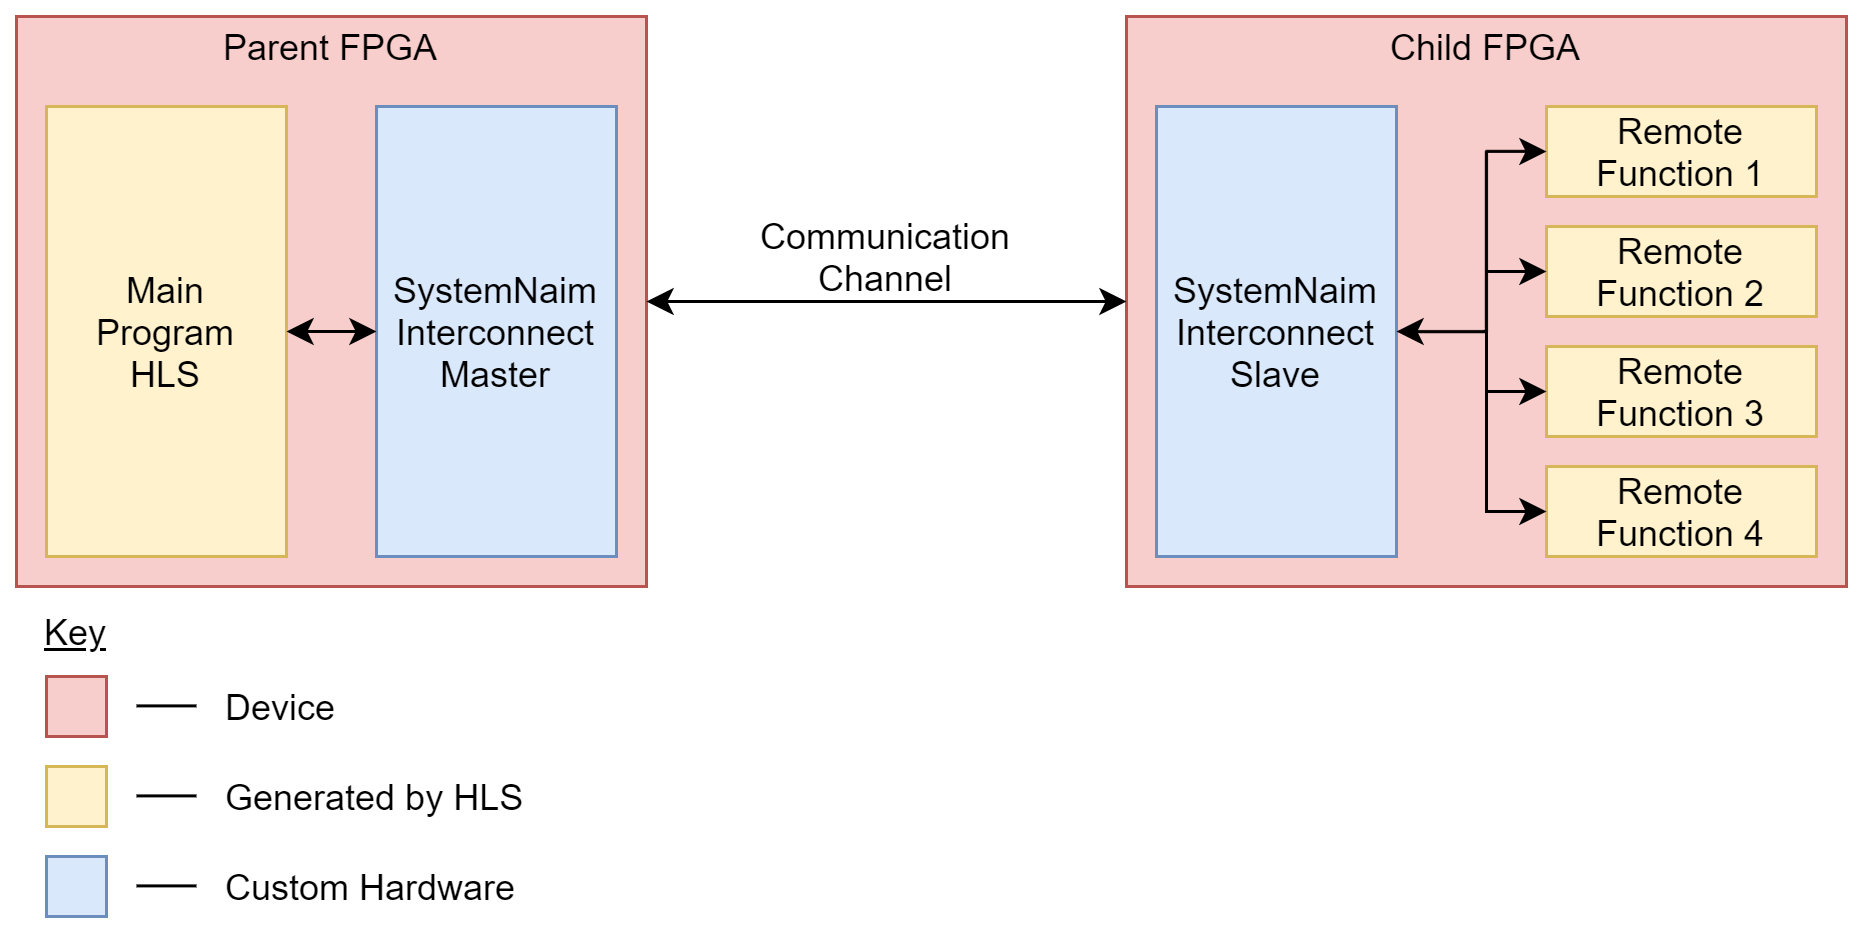
\includegraphics[width=0.9\textwidth]{03_design/images/full_system.png}
    \caption{Basic multi-FPGA system generated by SystemNaim}
    \label{fig:full_sys}
\end{figure}

To make it easier to understand the usage of the SystemNaim a design flow graph has been created, \autoref{fig:design_flow}. As can be seen, the user needs to provide input files, and then, using Quartus and the NIOS II development tools, load their system onto an FPGA.

\begin{sidewaysfigure}[!htb]
    \centering
    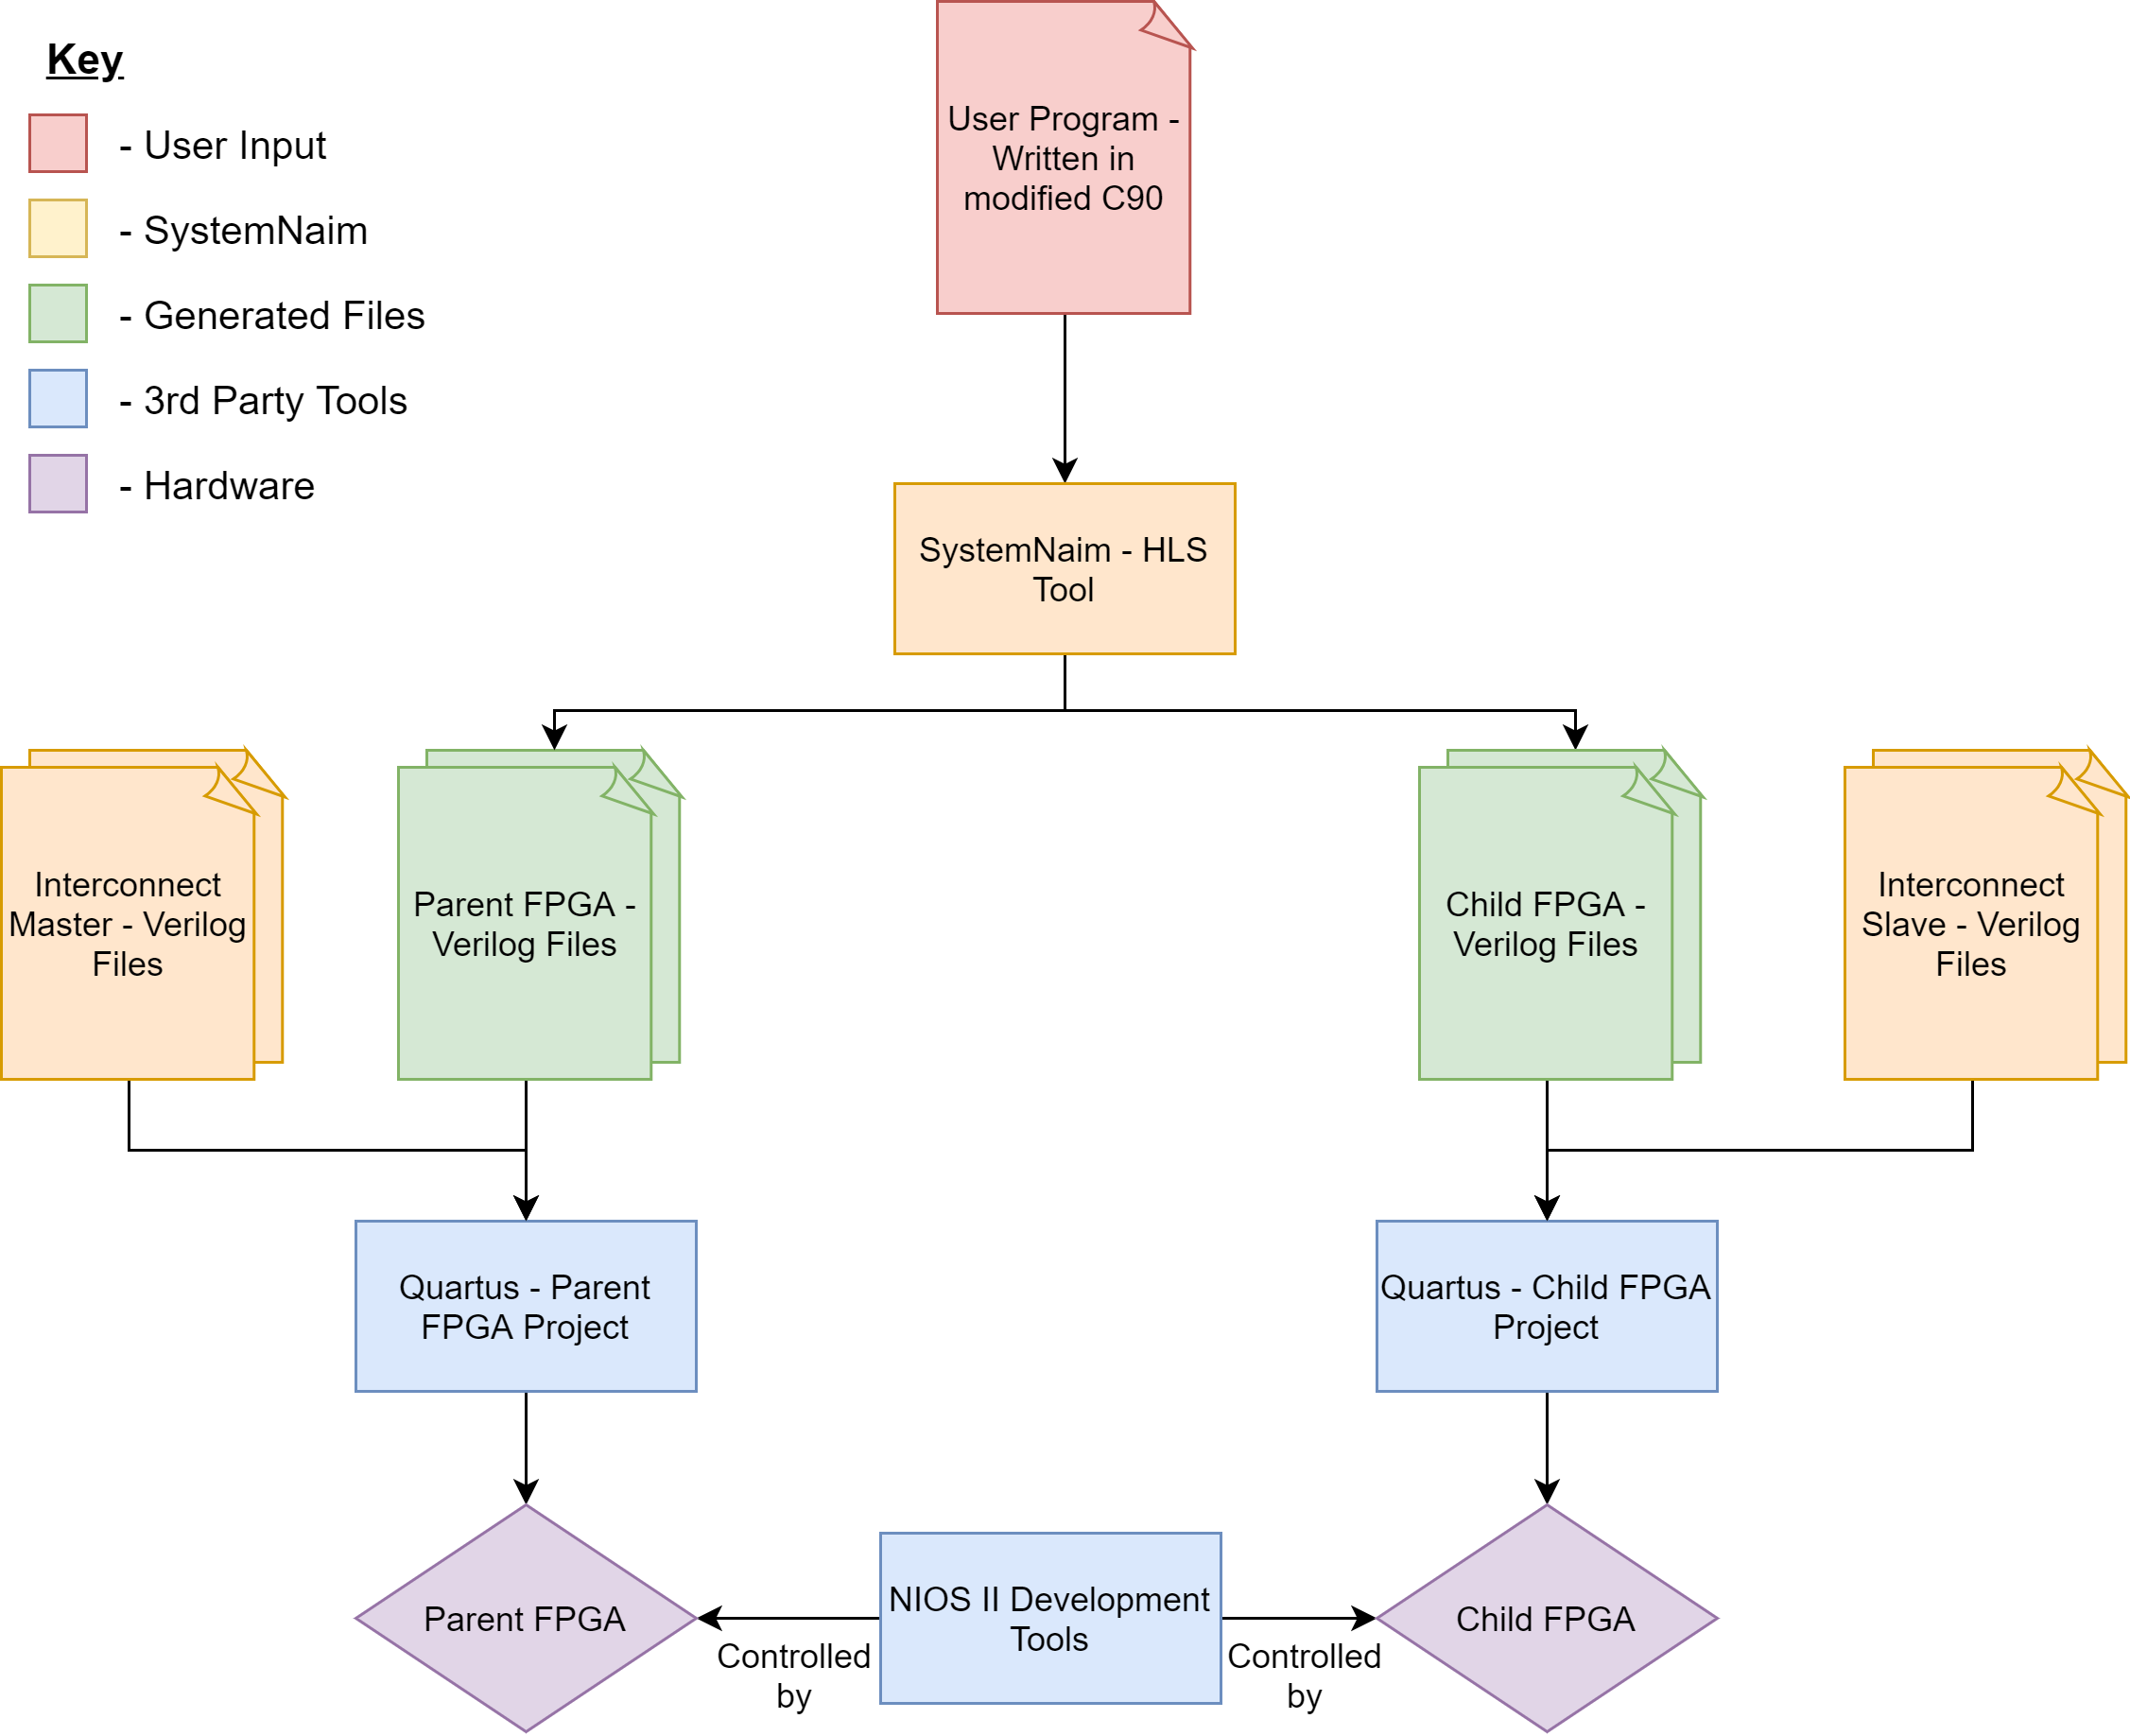
\includegraphics[width=0.9\textwidth]{03_design/images/design_flow.png}
    \caption{Design Flow of a system when using SystemNaim}
    \label{fig:design_flow}
\end{sidewaysfigure}
    \chapter{Future Work}

Given that SystemNaim was a final year project, and as such we could only put about 9 months of time into it, there are a lot of features that we would have like to have added or expanded upon. This section will go through some higher priority additions that weren't able to be made due to time constraints, but if added would make SystemNaim into a more complete and useful tool.

\section{Actual 'Multi'-FPGA System}

Currently, SystemNaim only allows for two FPGAs to communicate, one parent and one child. Allowing for more FPGAs to be used in tandem would give users the ability to exploit more parallelism within their programs, however it would also come with additional difficulties. The first challenge would be adding an addressing system so that each child FPGA could be identified. It would be likely that the system would just expand, with each child FPGA holding a collection of functions that could be called upon by the parent FPGA when required by the program. The parent FPGA would need to be able to, not only choose the correct function opcode, but also the correct address so that it could call the off-chip function it required. 

This could be added to the remote modules, which are instantiated on the parent FPGA, with each being configured at runtime to signal which child FPGA contains their function. The interconnect would then need to signal to the channel which child FPGA to deliver this command and opcodes to. With SPI this is pretty straightforward, every child FPGA would be connected to the same MISO and MOSI channel and  each would have their own SS\_EN (Slave Select Enable) signal, which would be asserted, by the parent FPGA, when that child FPGA was receiving a transaction. In the case of multiple off-chip functions being called at the same time, there would have to be a queue and the parent FPGA would call each function sequentially. Once it had finished calling all the necessary off-chip functions, it would then need to poll each of the activated child FPGAs, until their processing was complete, to return the result.

The polling, in this case, would likely be done in a round-robin fashion. With each child FPGA being sent a polling transaction, as described in IMPLEMENTATION SECTION, in order until all results had been returned. This does have the potential of causing latency spikes for the entire system. As was explored in \autoref{sec:interconnect}, missing a polling transaction can result in a large amount of additional latency, especially at low SPI Clock speeds, and adding multiple child FPGAs the parent needs to poll can only increase the worst case of a child FPGA missing a polling transaction. The solution for this would be to either know the latency of the off-chip functions, and only poll that child FPGA when it is assumed to have finished computation, or switch to a communication channel where both parties can start a transaction, such as Ethernet.

\subsection{Ethernet}

An Ethernet communication channel would allow child FPGAs to return data to the parent FPGA without the need for constant polling. Furthermore, only one port is required per device, with this never increasing as the system grows larger, and Ethernet can operate at a higher channel bandwidth than SPI thus further reducing the total overhead latency. The downside comes from the added complexity required in SystemNaim's custom hardware. Ethernet requires each device to be identified by a 48-bit number(MAC address) which cannot be assumed to known at runtime, therefore the parent FPGA would initially need to broadcast a request to all child FPGAs, for them to send an Ethernet packet containing their MAC address. As the parent FPGA receives these packets, they would need to store them in a lookup table to be able to communicate later on with the child FPGAs.

The additional effort required to get an Ethernet communication channel working would be worth-while as the added channel bandwidth plus capability for larger systems, could allow SystemNaim to implement more latency critical programs as well expand the scope to, in the future, allowing computation on the cloud.

\subsection{Changes to the HLS}

When allowing for systems with 3+ FPGAs a decision has to be made as to whether the user should decide which off-chip functions go on which child FPGA. The essence of SystemNaim is to give the user as much control over the end product as possible and merely remove the tedious hardware development aspects, and thus we'd likely incorporate a method that allowed the user to choose which functions are called on which FPGAs. An example of how this is possible is shown in \autoref{fig:multi_fgpa_hls}. Inspiration was drawn from the C++ STL, with the number between the “<>” symbol representing which child FPGA the function would be placed on (0 could mean the function should be run on the parent FPGA). Off all the challenges that would likely be faced when implementing this addition, the modification to the software side is probably the least difficult in a technical sense, however, the final decision on its implementation will define how users interact with this aspect of the system, and thus it is worth conducting a design investigation if there are any plans to ever add this feature in the future.

\begin{figure}[!h]
    \centering
    \begin{minipage}{0.5\textwidth}
    \begin{minted}{c}
split_fpga{
    holda = <0>hls_test_func_a(h, n);
    holdb = <1>hls_test_func_b(h, n);
    holdc = <2>hls_test_func_c(h, n);
    holdd = <3>hls_test_func_d(h, n);
}
    \end{minted}     
    \end{minipage}
    \caption{Method of allowing user to dictate which child FPGA a function is called on}
    \label{fig:multi_fgpa_hls}
\end{figure}

\section{General HLS Optimizations \& Additions}

\begin{itemize}
    \item Adding pipelining, FIFO's, arrays and maybe even giving the user access to FPGA pins
    \item Maybe even the off-chip function can start to use FPGA pins
\end{itemize}

As discussed in \autoref{sec:usability} the main downside of SystemNaim is the increase in latency of the hardware it produces, and as explained in DESIGN SECTION the decision to not spend too much time on creating optimal hardware was an intentional one. However, if SystemNaim were to be improved on in the future, optimizing the HDL generated by the HLS would make it much more appealing when compared to creating a dedicated hardware system. Below is a list of different optimizations and additions that could be made to SystemNaim's HLS aspect so that a user could create lower latency or more complex systems.

\subsection{Loop Pipelining}

Pipelining is an example of an optimization that would drastically reduce the latency of any loop-based function. In essence, pipelining allows for multiple iterations of a loop to be computed at the same time and is especially useful when a single iteration may take many cycles. However, in order to implement this feature correctly SystemNaim would need to be able to detect data dependencies both within an iteration and between iterations, and thus an extra step of analysis in the tool would need to be added. 

To illustrate the benefit of loop pipelining, a small example will be looked at. Imagine if we had a loop with 100 iterations and each iteration took 5 cycles. To compute this loop fully would require 500 cycles, with no pipelining. To calculate the latency of this loop with pipelining we need to use the formula found in \autoref{eqn:pipelining}. Initiation interval (II), a term that we haven't used yet, is a defined as the number of cycles between the start of each iteration of the loop. For an unpipelined loop the II is equal to the latency of each iteration. If we were to have an II of 1, the best case, the example loop would only take 104 cycles to compute, thus giving a large reduction in latency. With how prevalent loops are in modern programming, adding this feature would benefit a lot of programs that may be implemented using SystemNaim, but would require an overhaul of the line-to-state model currently in use in order to allow for concurrent hardware.

\begin{equation}
    L_{tot} = L_s + I * (N - 1) \label{eqn:pipelining} 
\end{equation}
where:
\begin{conditions}
L_{tot}    &  is the total latency of the loop \\
I    & is the Initiation Interval(Throughput) \\
N & is the total number of iterations in the loop \\
L_s & is the latency of a single iteration
\end{conditions}


\subsection{FIFO's \& arrays}

In \autoref{sec:dedicated_hardware_computation}, a case when a FIFO would be optimal instead of a loop was given. FIFO's have a lot of uses in hardware design, especially when it comes to acting as the middle man between data-producing and data-consuming hardware modules. They can allow for multiple pipelined loops to act concurrently, without consuming a large amount of resources, and can act as queues for feeding data into a function. Giving access to this hardware construct to users of SystemNaim would allow them to create more complex and optimal systems. This would be the same with arrays, which allow for more complex algorithms to be implemented in SystemNaim. 

Being able to store data is of vital important when creating a modern system, however, when deciding what features SystemNaim needed to implement to prove our aims we realized arrays weren't necessary. Nevertheless, in the future adding both of these constructs would vastly increase the versatility of SystemNaim, but not without their share of challenges. For arrays, multiple sources accessing the same part of memory would require multiplexers so that there wouldn't be any contention, which poses the risk of increasing the latency of each access. In terms of FIFO's, the challenge is more on the HLS side. Giving access to all aspects of the FIFO to the user would be tricky without using a class-based method inspired by C++'s OOP. This would result in potentially too large of a change in syntax, and at that point, instead of making changes to the base C language, it would be worth switching SystemNaim's base language to C++. The additional work while large, could open up more possibilities for different hardware modules to be added in the future, with member functions being the designated way of controlling and interfacing with them.

Each addition would require a large amount of work but definitely has merits, and what would be achievable within SystemNaim after they had been added would be very interesting to investigate

\subsection{FPGA Pins}

The final addition that we believe SystemNaim would benefit from, is the ability for users to access FPGA pins from their top-level function. Pins on an FPGA are use as I/O and allow for external data streams to be processed on the FPGA. They are essential for most real world FPGA use cases, and giving users the ability to interface with external devices would make SystemNaim a more versatile tool. Users would be able to stream in data from an Ethernet or USB port and user their multi-FPGA system as an accelerator within a larger system. 

Instead of giving access directly to the pins themselves, which would breach the software vs hardware programming paradigm and would defeat the purpose of an HLS tool, we could allow for FIFO's to be implemented at the top-level and then expect the user to develop some hardware to get the data from their external source into said FIFO. This would, of course, require some hardware proficiency on the user's behalf, but it would still give increase the use case of SystemNaim. It would be of interest to actually perform an investigation into the possibility of requiring no hardware proficiency from a user, but still giving them access to I/O pins and ports within the HLS tool.

Another benefit of such a feature would be for child FPGAs to also be able to access their own I/O pins, and thus would be able to consume data from their own sources rather than being given it by the parent FPGA. From \autoref{sec:interconnect}, we know that this would reduce the transfer overhead if we no longer need to send data operands across the channel, therefore, further reducing the latency of the total system.

\section{Inter-FPGA Data Streaming}

\begin{itemize}
    \item Potentially you could stream data through the channel in order to get more than two operands across.
    \item You could also split the channel into two. One for starting off-chip functions and one for streaming data between the FPGAs.
\end{itemize}

    \chapter{Evaluation}
\label{chp:eval}

Evaluation is an important part of deciding whether SystemNaim achieved its aims \& goals. The following sections discuss: interconnect performance, program affinity and usability of SystemNaim, and attempt to gain insight into the issues or benefits produced by the tool.

\section{Interconnect Performance}
\label{sec:interconnect}

Calling a function implemented in hardware off-chip is not latency free. There will be some overhead latency associated with packaging the data to be sent over the channel, sending the data over the channel itself, and then repeating this process in order to return the data produced by the off-chip function back to the main FPGA. Therefore, it is of importance to measure this overhead so that we can gauge the efficiency of the interconnect hardware that was designed for SystemNaim.

Since the decision was made to implement an SPI communication channel for the final product, we had to into consideration the SPI clock speed used by the system. On an SPI channel, a single bit is sent on every cycle of the SPI clock meaning it takes 32 SPI Clock cycles to send single 32-bit integer. Increasing the SPI Clock speed allows for a higher performing channel, which is able to send data in a shorter period, however, this increase comes at the cost of reliability. This section explores the effect of the SPI Clock rate on a test system. We will attempt to prove that increasing the clock speed does reduce the total overhead, but will also investigate the overhead added from the interconnect to the latency of the system.

\subsection{Mathematical Model for Overhead Latency}

In order to find out how much of the latency of a multi-FPGA system, created in SystemNaim, can be attributed to the interconnect, we must first devise a model that can tell us what data needs to be gathered. At it's most simple, we can model the latency of a system as the sum of the time taken to perform the actual processing i.e. the code that the user entered into the tool, and the time taken to encode, transmit, receive, and decode the data across the SPI channel i.e. the overhead. \autoref{eqn:tot_sys_latency}, shows the mathematical equivalent of the previous statement.

\begin{equation}
    L_{sys} = L_{processing} + L_{overhead}
    \label{eqn:tot_sys_latency}
\end{equation}

In order to find $L_{processing}$ from \autoref{eqn:tot_sys_latency} we make the following assumption: the total processing time, in cycles, for a multi-FPGA system is the same as a single FPGA system where both the off-chip function and on-chip function, from the former system, are run in parallel. In essence, if we measure the latency of a system that has been created on a single FPGA using SystemNaim's “split” keyword then we can assume the total latency of this system is equal to $L_{processing}$ for a multi-FPGA system where “split” has been replaced with “split-fpga”.

Before we continue an important side note, $L_{rest}$ will refer to the latency caused by the processing outside the function call i.e. the processing before and after the function call. We can assume this because SystemNaim generates the exact same hardware in both the single FPGA and multi-FPGA case before and after the function call. Furthermore, for simplicity the single FPGA system with parallel hardware will be called the Multi-Thread Single Chip (MTSC) system, as it denotes parallel computation on a single chip, likewise, the multi-FPGA system will be referred to as the Multi-Thread Multi-Chip (MTMC) system. 

We can prove that $L_{processing} = L_{MTSC}$, where $L_{MTSC}$ is the total latency for an MTSC system, if we place the following constraint on the system: all parallel functions in the system must have the same latency.

\autoref{fig:multi_func_call} is a diagram representing the program path for a multi-function call in an MTSC system. As can be seen the total latency $L_f = max(L_1,L_2)$, however with our constraint $L_1 = L_2$, and thus we can simplify to \autoref{eqn:fcl_2}. \autoref{fig:multi_fpga_call} shows a similar diagram for the MTMC case. Assuming both functions are the same and that $L_{I1} > 0 \text{and} L_{I2} > 0 $ then equations \ref{eqn:mtmc_latency_start} to \ref{eqn:mtmc_latency} hold. 

\begin{align}
    &L_{f\_MTSC} = L_1 \label{eqn:fcl_1} \\
    &L_{MTSC} = L_{rest} + L_1 \label{eqn:fcl_2}
\end{align}

\begin{align}
    &L_{f\_MTMC} = max(L_1 + L_{I1} + L_{I2} , L_2) = L_1 + L_{I1} + L_{I2} \label{eqn:mtmc_latency_start} \\
    &L_{MTMC} = L_{rest} + L_1 + L_{I1} + L_{I2}  \\
    &L_{MTMC} = L_{MTSC} + L_{I1} + L_{I2} \\
    \therefore \; &L_{processing} = L_{MTSC} \label{eqn:mtsc_processing} \\
    \& \; &L_{overhead} = L_{I1} + L_{I2} 
    \label{eqn:mtmc_latency}
\end{align}

Given those results we prove that we can use the MTSC latency in the MTMC calculations. We also proved that the overhead was $L_{overhead} = L_{I1} + L_{I2}$, which represents the latency incurred by sending and receiving data over the channel and seems like a sensible representation of the overhead. Furthermore, \autoref{eqn:overhead_formula} show's that we can calculate the overhead latency by finding the difference between the latency of an MTMC and MTSC system, provided that they both call the same functions and have the same processing before and after the function call. In SystemNaim this is easily doable by switching the “split” keyword with “split-fpga”. 

\begin{align}
    &L_{MTMC} = L_{processing} + L_{overhead} \\
    &L_{overhead} = L_{MTMC} - L_{processing}  \\
    &L_{overhead} = L_{MTMC} - L_{MTSC}\label{eqn:overhead_formula}
\end{align}

\begin{figure}[!htb]
    \centering
    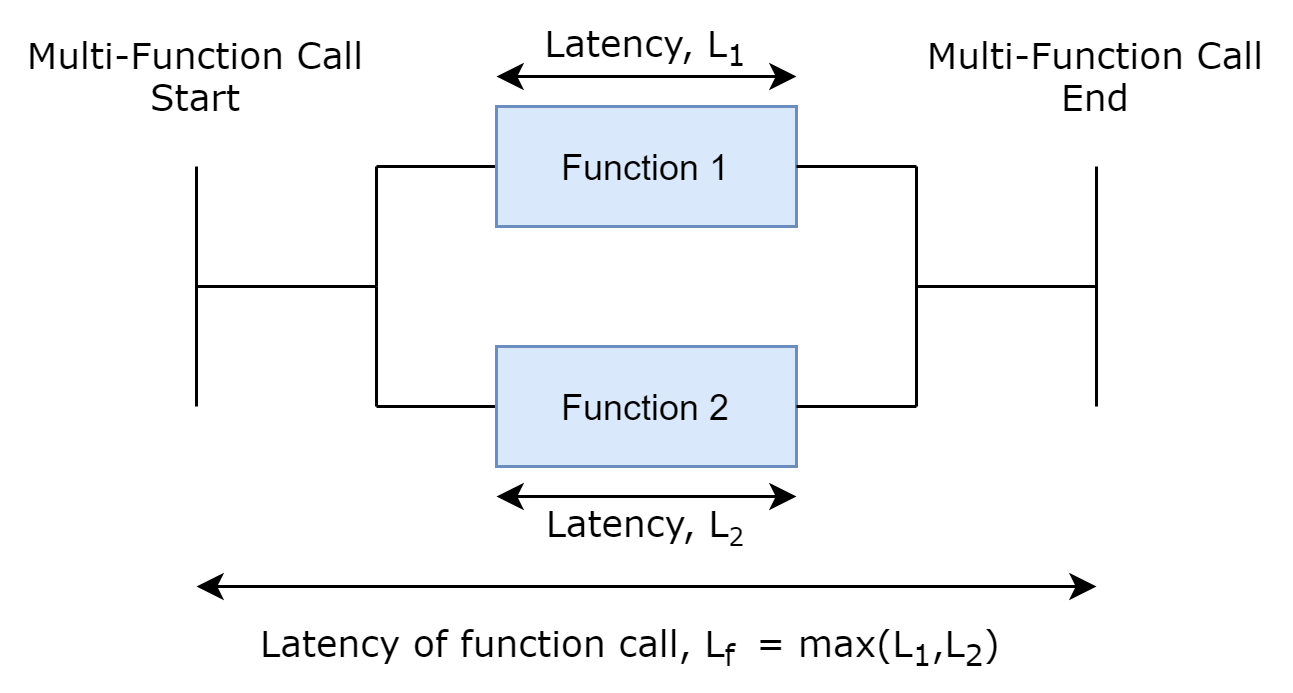
\includegraphics[width=0.9\textwidth]{05_evaluation/images/concurrent_latency.png}
    \caption{Latency of single FPGA multi-function call}
    \label{fig:multi_func_call}
\end{figure}

\begin{figure}[!htb]
    \centering
    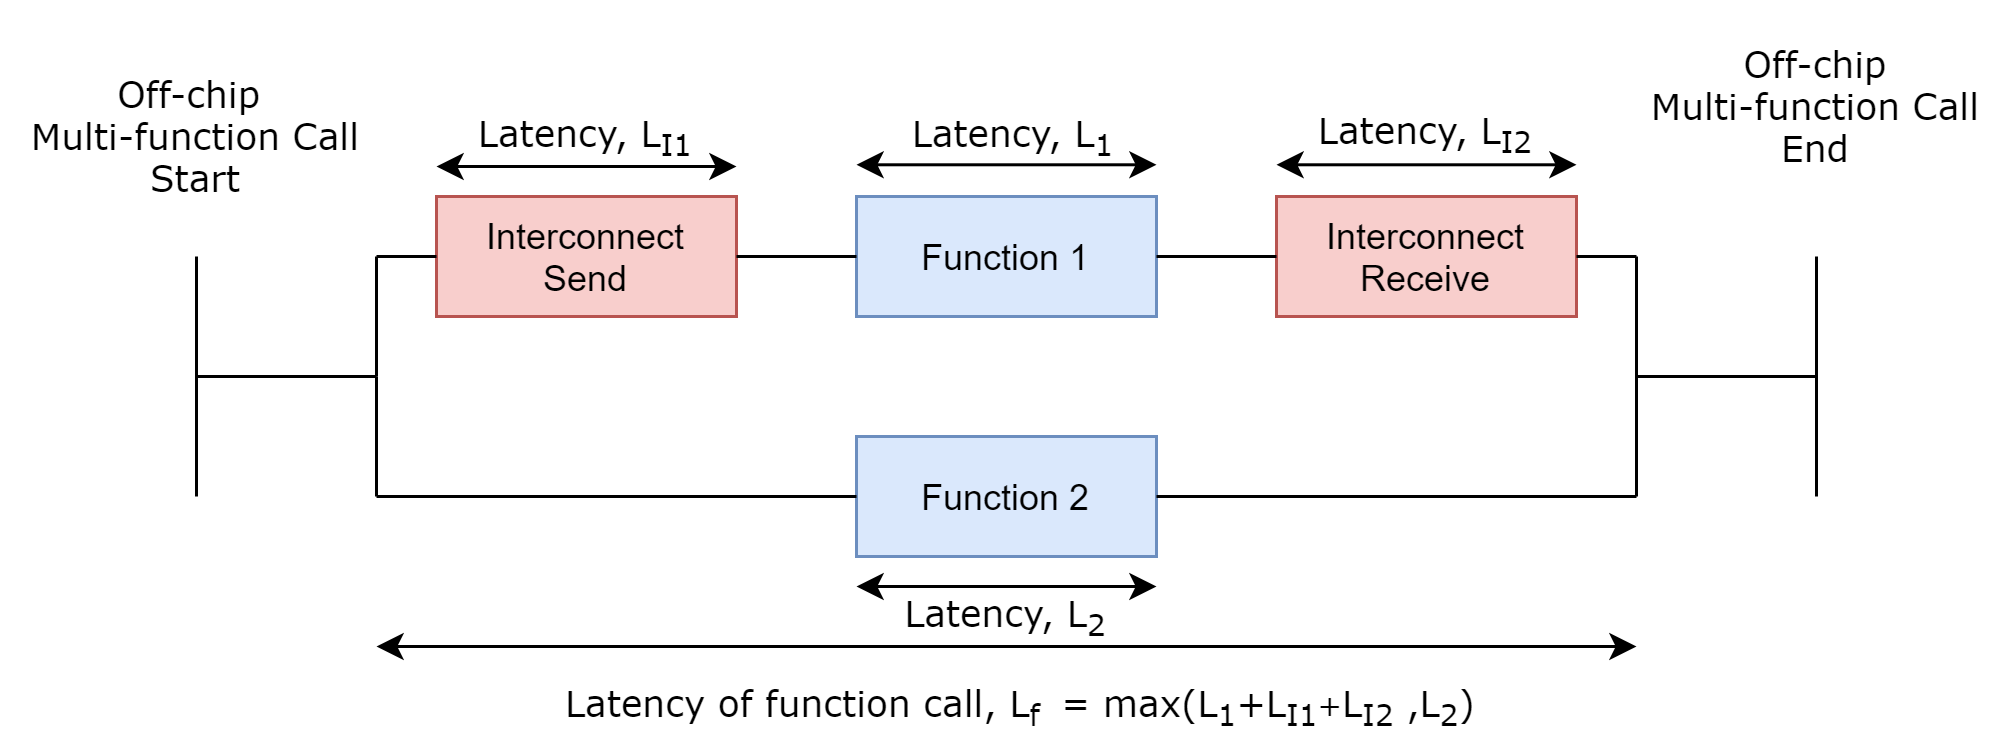
\includegraphics[width=0.9\textwidth]{05_evaluation/images/offchip_latency.png}
    \caption{Latency of multi FPGA multi-function call}
    \label{fig:multi_fpga_call}
\end{figure}

\subsubsection{Channel Bandwidth}
 
We can further dissect the overhead latency and split it into two parts. The transfer overhead, $L_{t\_overhead}$, which is latency cost incurred for transmitting and receiving data over a channel and the interconnect overhead, $L_{i\_overhead}$, which is the latency cost from encoding and decoding the data transmitted. Essentially, the latter part comes from the hardware designed specifically for SystemNaim, whereas the former is merely the limit of the channel. In an ideal world the interconnect overhead would be 0 and only the transfer overhead would exist. 

We can calculate the transfer overhead by knowing the rate at which data is transferred over the channel, and in the case of an SPI channel this is dependent on the SPI clock speed, $\mathit{SPI}_{clock}$. The SPI clock speed is different from the system clock speed, $\mathit{SYS}_{clock}$; both can be configured by the user but in our case we have a variable SPI clock speed and a static system clock speed at 50MHz.

Our SPI channel transfers data at 1 bit per SPI clock cycle, which is standard, however we're not interested in how long it takes for data to be transferred relative to the SPI clock. Instead, we would like to know how many system clock cycles it takes to transmit a single bit. We'll refer to this value as the channel latency, $L_{channel}$, and it can be calculated by dividing the system clock speed by the SPI clock speed. The resulting value has a unit of cycles per bit.

For SystemNaim, we know that any off-chip function call requires 128 bits of data to be sent over the channel. 96 bits (or 3 integers) are required to send the opcode, operand A and operand B, while the last 32 bits are for the data that needs to be returned to the main FPGA. Therefore, the formula for the transfer overhead, which is measure of how many clock cycles it takes to transfer all the data over a channel for an off-chip function call, is shown in \autoref{eqn:overhead}. 

\begin{equation}
    L_{channel} = \frac{\mathit{SYS}_{clock}}{\mathit{SPI}_{clock}} 
    \label{eqn:clock_speed}
\end{equation}

\begin{equation}
    L_{t\_overhead} = 128 * L_{channel}
    \label{eqn:overhead}
\end{equation}

\subsection{Test model}

With the maths and the modelling in place we can now begin testing the system to see if we can get an experimental value for the overhead and how it is affected by the SPI clock speed. For this test we use a program which calls 2 function, which are syntactically the same, and then exits. We first compile the program with both functions being called within a “split” block and test the latency of this MTSC system. Afterwards we test the same program, but we replace the “split” keyword with the “split-fpga” keyword, this will be the MTMC system. 

The MTMC system will be run multiple times with varying SPI clock speeds, and for each test we will compare the latencies between the MTMC and MTSC systems, compute the transfer overhead and find the interconnect overhead.

\subsection{Results}

\autoref{tbl:spi_clk_results} shows the data gathered, in accordance to testing methodology laid out above. It should be noted that the \textbf{Channel Latency} and \textbf{Est. Transfer Overhead} columns have been calculated using no gathered data. Both columns are dependent on the \textbf{SPI Clock (Hz)}, and the calculations for each can be found in Equation \ref{eqn:clock_speed} and \ref{eqn:overhead} respectively.

\autoref{fig:spi_clk_graph} is a summation of the important data from the table in the form of graph, thus making it easier to identify trends in the data.

\begin{sidewaystable}
    \centering
    \begin{threeparttable}
    \begin{tabular}{l|l|l|l|l|l}
    \textbf{SPI Clock (Hz)} & \textbf{Channel Latency} & \textbf{Latency (Cycles)} & \textbf{Overhead (Cycles)} & \textbf{Transfer Overhead} & \textbf{Interconnect Overhead} \\ \hline
     125,000               &  400                 &  52,918              &  52,794              & 51,200                &  1,594                                      \\
     250,000               &  200                 &  26,518              &  26,394              & 25,600                &  794                                        \\
     252,525\tnote{*}      &  198                 &  26,254              &  26,130              & 25,344                &  786                                        \\
     277,777\tnote{*}      &  180                 &  23,878              &  23,754              & 23,040                &  714                                        \\
     312,500               &  160                 &  26,532              &  26,408              & 20,480                &  5,928                                      \\
     347,222\tnote{*}      &  144                 &  23,892              &  23,768              & 18,432                &  5,336                                      \\
     500,000               &  100                 &  16,632              &  16,508              & 12,800                &  3,708                                      \\
     1,000,000             &  50                  &  8,382               &  8,258               & 6,400                 &  1,858                                      \\
     1,923,076\tnote{*}    &  26                  &  4,422               &  4,298               & 3,328                 &  970                                        \\
     5,000,000             &  10                  &  1,782               &  1,558               & 1,280                 &  278                                        \\
     8,333,333\tnote{*}    &  6                   &  1,122               &  998                 & 768                   &  230                                        \\
     12,500,000            &  4                   &  792                 &  668                 & 512                   &  156                                        \\
     25,000,000            &  2                   &  542                 &  418                 & 256                   &  162                                       
    \end{tabular}
    \begin{tablenotes}\footnotesize
        \item[*] These values for SPI clock speed are not factors of the system clock, and are actually irrational.
        \end{tablenotes}
    \end{threeparttable}
    \caption{Effect of SPI clock speeds on overhead latency}
    \label{tbl:spi_clk_results}
\end{sidewaystable}

\begin{figure}[!htb]
    \centering
    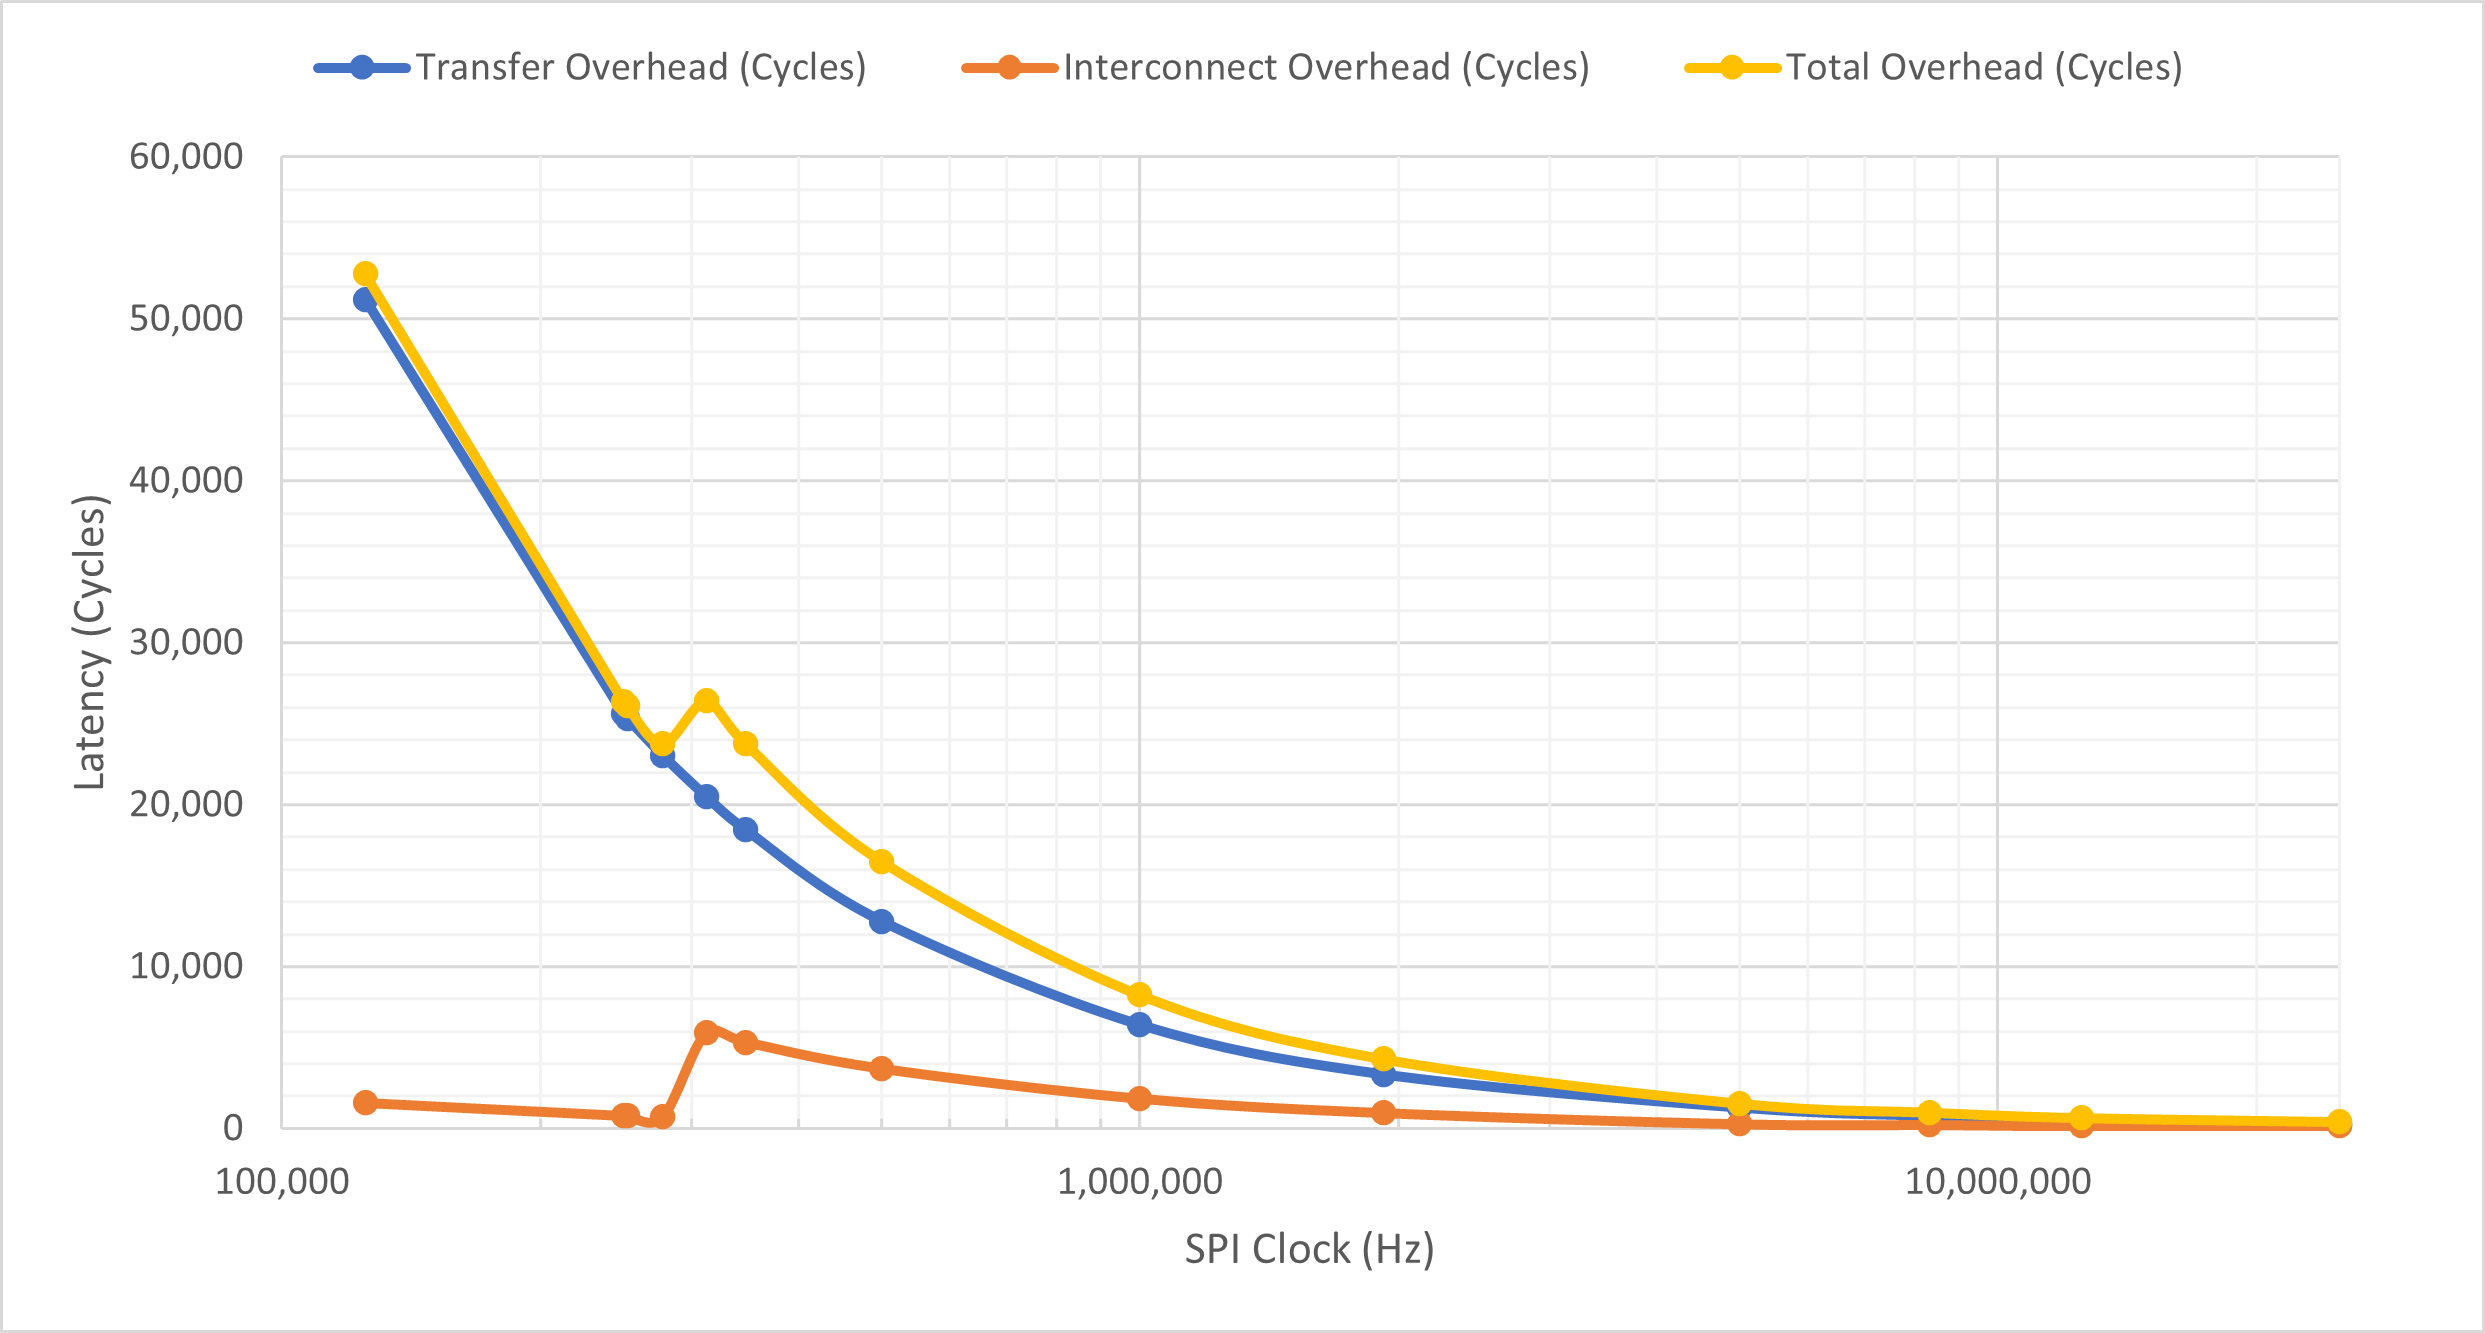
\includegraphics[width=0.9\textwidth]{05_evaluation/images/overhead_vs_spi_clk.png}
    \caption{Overhead Latency vs. SPI Clock Speed \textit{(Best case would be that the total overhead equals the transfer overhead)}} 
    \label{fig:spi_clk_graph}
\end{figure}


\subsection{Conclusions}

Generally speaking, we can conclude that as we increase the SPI clock speed the total overhead latency decreases, we can also deduce that the main proportion of the overhead is transfer overhead. This is supported by \autoref{fig:spi_clk_graph}, and was the result we intended for this investigation to prove. However, there are a few interesting caveats to this conclusion that we cannot ignore. Firstly, while not shown on the graph or table, during testing it was found that setting the clock speed the values higher than 8MHz resulted in increased channel instability. Tests would occasionally fail to complete with transactions not being detected by either the on-chip or off-chip interconnect, the higher the clock speed the more likely this phenomenon would occur.

This instability may have been caused by the physical components of the channel not being able to accurately keep up with these speeds. For the final product GPIO pins on both FPGAs were connected using breadboard jumper cables, which aren't intended to be used for data communication. Potentially, at clock speeds of 8MHz and above, the GPIO pins were not able to go from high to low, and vice versa, fast enough to generate a detectable clock on the child FPGA. The fault could also lie with the SPI core and the FPGA hardware. The SPI core takes in the main system clock, generates the SPI Clock and transmits that signal to a GPIO pin. Therefore, there may be an issue between the pin and the FPGA hardware. Unfortunately, there's no way to be certain of the cause, and instead we can only conclude that speeds above 8MHz result in unreliable performance. 

The more interesting result from the gathered data, however, comes from the trend of the \textbf{Interconnect Overhead}. While it would be expected that the latency from the interconnect would be generally static, with only minor fluctuations since the task of encoding data should be uniform, what we see instead is a generally decreasing trend except for a steep rise in latency at 312,500Hz. This behaviour, however, makes complete sense given the design of the interconnect and is a consequence of the SPI channel only allowing the master to initiate transactions. 

As explained in \autoref{sec:impl_interconnect}, the child FPGA cannot indicate to the parent FPGA when it has completed processing its off-chip function. Therefore, in order to receive the return data the parent FPGA must continuously send polling transactions on the SPI channel. Because of this, when the off-chip function is complete, and it passes the result to the SPI slave core, the core must wait for the current polling transaction to finish before the next one starts, and then it can send the valid return data. Therein lies the issue, the wait for a current transaction to finish.

The worst case for this scenario is if the slave SPI core has to wait for a full transaction, minus one cycle, to complete before it can send its data. At lower clock rates this can take thousands of cycles, more specifically $32 * L_channel$ cycles, since each transaction consists of 32 bits. Furthermore, how close the end time of an off-chip function is to the end of any given polling transaction is dependent on both the SPI clock speed and the latency of the function itself, therefore it becomes incredibly difficult to avoid the worse case scenario and the interconnect overhead becomes stochastic in nature. However, we can minimize the interconnect overhead by increasing the SPI clock speed, as this reduces the number of system cycles it takes for a polling transaction to finish and thus also the number of system cycles the slave SPI core has to wait in the worse case scenario.

In conclusion, we should try to maximize the SPI clock speed as this reduces the transfer overhead, and minimizes the worst case for the interconnect overhead, thus, increasing the performance of the MTMC system.

\section{System Performance}
\label{sec:sys_perf}

Now that we have established that higher SPI clock speeds, and also higher channel bandwidths, reduce the total overhead associated with calling a function off-chip, we can start to explore what kind of programs can exploit the benefits of a multi-FPGA system the best. In general, FPGAs are mainly used for their ability to exploit parallelism in programs, and the motivation for using multiple FPGAs in tandem is to access more resources (LUTs, BRAM, DSPs etc.). Therefore, it stands to reason that the best programs to run on a multi-FPGA system are one which can have large parts of the processing run in parallel but also require a large amount of resources.

Considering the limitations of SystemNaim it would be difficult for us to write programs which take up a large percentage of an FPGAs resources, however, we can investigate how well we can exploit a program's affinity for parallelism and how the same program performs on a single FPGA system versus a multi-FPGA system. Ideally, we will be able to prove that as program latency increases the percentage contribution of the interconnect overhead to the total latency will decrease, thus, giving more credence to using a multi-FPGA system.

\subsection{Test Model}

The model for this investigation is relatively straightforward. We will write a numerical integration program and using SystemNaim, run the program on three different systems. The first will be a full sequential program with no parallelism, the second will exploit the parallelism of the program, but all processing will happen on a single FPGA, the final system will be a multi-FPGA one, which will also exploit the parallelism of the program but will also perform some processing on a second FPGA.

Borrowing from the previous investigation each system will have a short-hand to make them easier to identify. The sequential system will be the Single-Thread Single Chip (STSC) system, the single FPGA system with parallelism will be the Multi-Thread Single Chip (MTSC) system and finally the multi-FPGA system will be the Multi-Thread Multi-Chip (MTMC) system.

The program that we will be running will contain loops that run for a fixed number of iterations. As we vary the number iterations, we will measure the latency of each system at each step and compare the results. Furthermore, we will dissect the MTMC latency into processing latency and overhead, where the overhead is a measure of the cost incurred, in cycles, for perform part of the processing off-chip.

As a final note, the SPI core in this investigation will be set at 5MHz or 10\% of the system clock. This decision was made in order minimize channel latency, while maintaining reliability.

\subsection{Numerical Integration Program}

The numerical integration method that we decided to implement was the Composite Simpson's rule, which is shown in \autoref{eqn:comp_simp}. What makes this specific implementation interesting to us are the two sums, $s_1$ and $s_2$. These sums can be easily setup so that they are computed in parallel when implemented in SystemNaim. All that is needed is to make functions of each sum and call them within a “split” or “split-fpga” block to produce either an MTSC or MTMC system respectively. $n$, is also chosen by the user, and we can increase that to increase the number of total iterations the program must make.

Unfortunately, since a function in SystemNaim can only have two numerical inputs there are some limitations on the program. The first is that $a$, the lower bound of the integral will be a compile-time constant, thus, unmodifiable during runtime. The second is that both functions will have knowledge of what $f(x)$ is at runtime, and will make calls to a function in software which computes the value of $f(x)$. Each of these calls in software will create a module in hardware, resulting in two hardware modules which compute $f(x)$. This, however, is necessary for the parallelism and will allow for some interesting analysis that will be explored later on.

The final issue is unrelated to the two input problem, but is due to SystemNaim not supporting floats. Only integers are supported and to ensure we produce valid results, care has been taken in order to choose $a$, $b$, $n$, and $h$ such that no decimal values are produced during operation.

Overall, none of the three issues disrupt the purpose of the investigation at hand, which focuses on how the latency of the systems are affected as we increase the number iterations the program has to run. However, in the interest of a fair and open investigation it was deemed important to include them.

\begin{align}
    & s_1(f(x),n,a,h) = 2 \sum_{j=1}^{n/2-1}f(x_{2j}) \text{, where } x_j = a + jh \\
    & s_2(f(x),n,a,h) = 4 \sum_{j=1}^{n/2}f(x_{2j-1}) \text{, where } x_j = a + jh \\
    &\int_{a}^{b} f(x) dx \approx \frac{h}{3} \Big[ f(x_a) + s_1(f(x),n,a,h) + s_2(f(x),n,a,h) + f(x_b) \Big] \text{, where } h = \frac{b-a}{n}  \label{eqn:comp_simp}
\end{align}

\subsection{Results}

\autoref{tbl:system_results} shows the results of the investigation. \autoref{fig:latency_v_iter} shows the same data but in the form of graph in order to be able to identify trends more easily.
Finally, \autoref{fig:overhead_percent} shows the percentage contribution of the overhead to the MTMC latency, however, this graph needs a slight amount of justification before we can draw conclusions from it.

The investigation has been designed in such a manner that the MTSC and MTMC systems are exploiting the same amount of parallelism in the program and are preforming the same amount of processing. The only difference is that the MTMC must also go through the trouble of calling a function off-chip, which has been proved to incur a latency cost. Therefore, we assume that the processing latency i.e. the amount of cycles spent executing the code that the user entered into the tool, are the same for both systems. Thus, the difference between the two latencies is the cost incurred to call a function off-chip and is therefore the latency. This was much more rigorously proved in the previous investigation but the reasoning above provides an adequate platform for this section.

Finally, by comparing the MTSC latency and the calculate overhead we can guage what percentage of the total latency of the MTMC system was due to the off-chip function call and thus evaluate whether the jump from single FPGA to multi-FPGA is worth the latency cost. 

\begin{sidewaystable}
    \centering
    
    \begin{threeparttable}
    \begin{tabular}{l|l|l|l|l|l}
    \textbf{Iterations ($n$)} & \textbf{STSC Latency} & \textbf{MTSC Latency} & \textbf{MTMC Latency} & \textbf{Overhead} & \textbf{STSC to MTMC Latency Reductions}\\ \hline
     200        & 2,572               & 1,370                 & 2,839                 &  1,469         &    -10.38\%    \\
     400        & 5,072               & 2,670                 & 4,215                 &  1,545         &    16.9\%    \\
     600        & 7,572               & 3,970                 & 5,591                 &  1,621         &    26.1\%    \\
     800        & 10,072              & 5,270                 & 6,967                 &  1,697         &    30.1\%    \\
     1000       & 12,572              & 6,570                 & 7,999                 &  1,429         &    36.4\%    \\
     1200       & 15,072              & 7,870                 & 9,375                 &  1,505         &    37.8\%    \\
     1400       & 17,572              & 9,170                 & 10,751                &  1,581         &    38.8\%    \\
     1600       & 20,054              & 10,470                & 12,127                &  1,657         &    39.5\%    \\
     1800       & 22,572              & 11,770                & 13,503                &  1,733         &    40.2\%    \\
     2000       & 25,072              & 13,070                & 14,535                &  1,465         &    42.0\%    \\                                 
    \end{tabular}
    \begin{tablenotes}\footnotesize
        \item Latencies are measured in cycles
        \end{tablenotes}
    \end{threeparttable}
    \caption{Effect of Program iterations on total latency}
    \label{tbl:system_results}
\end{sidewaystable}

\begin{figure}[!htb]
    \centering
    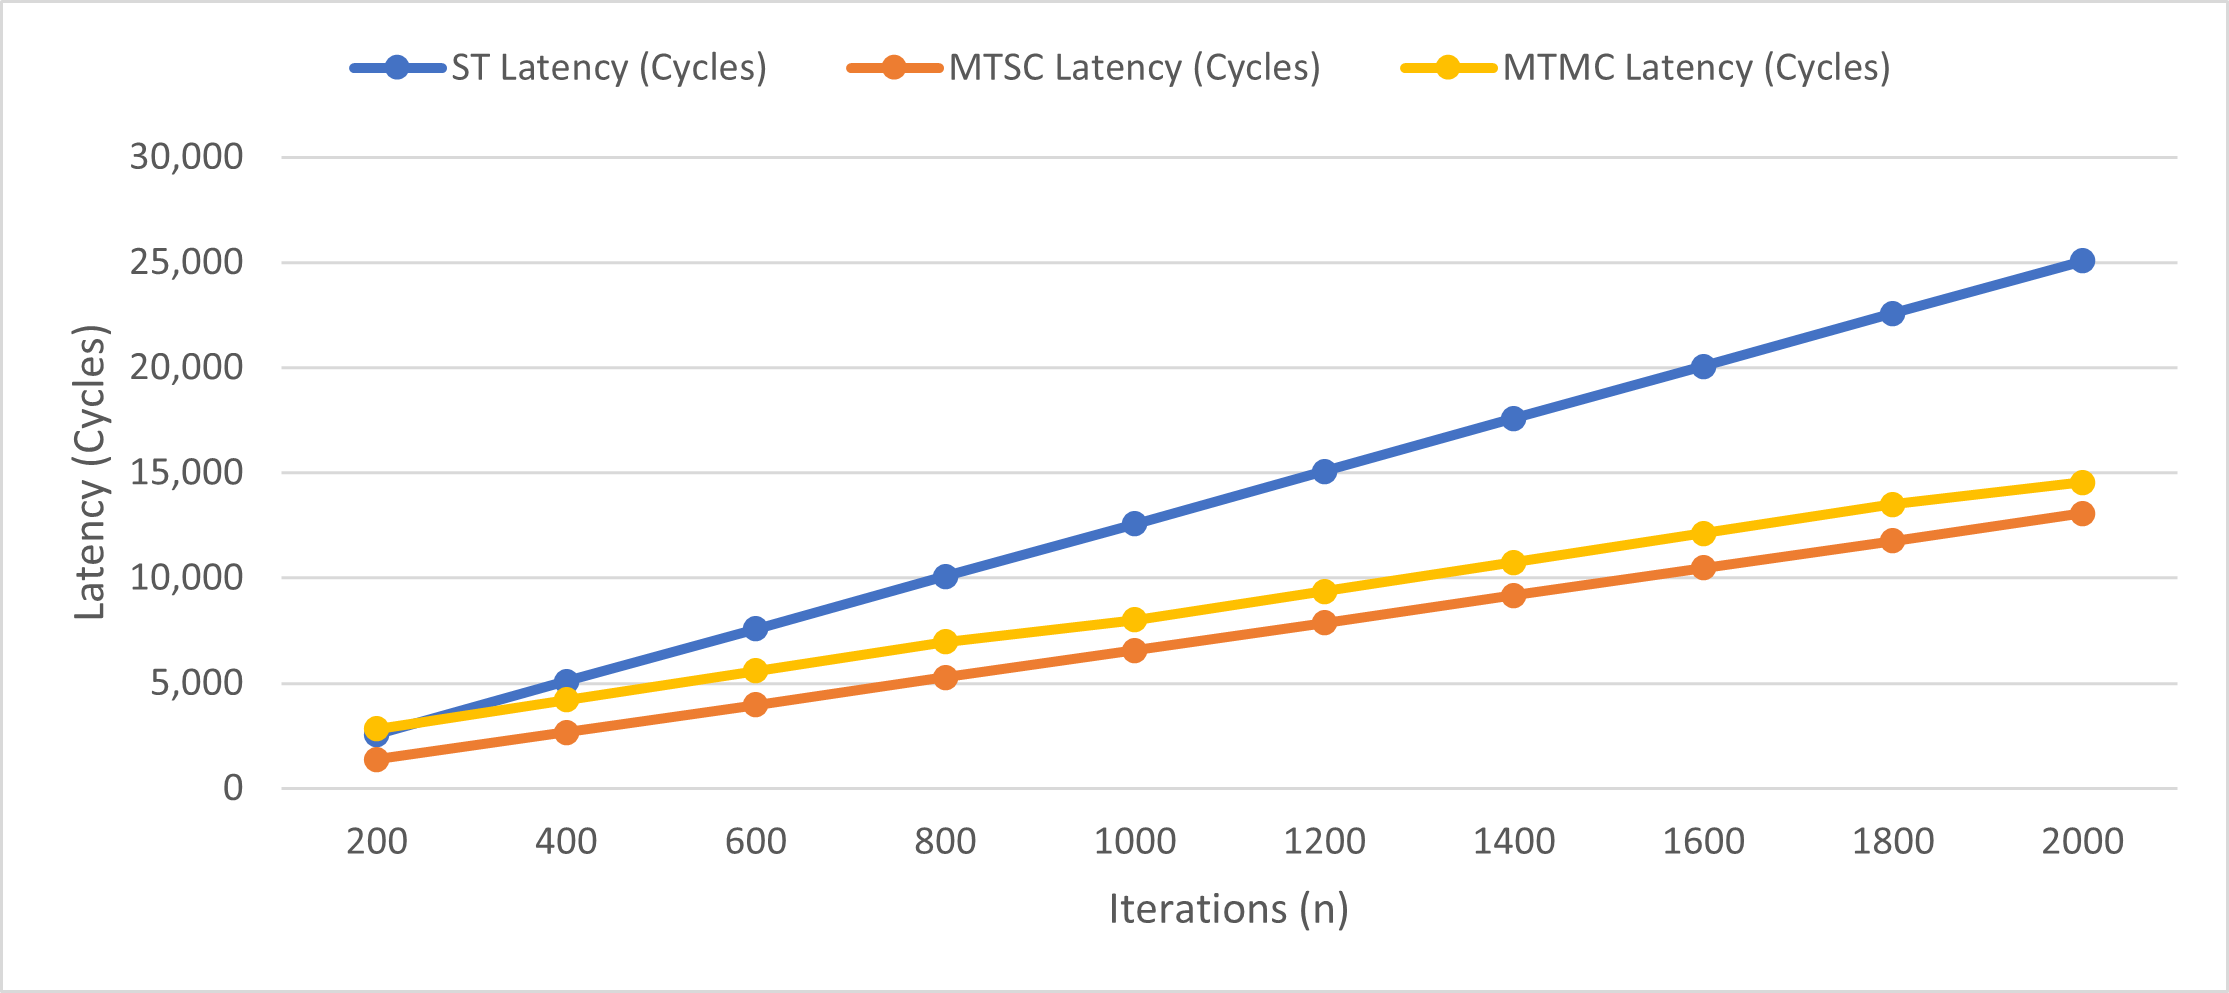
\includegraphics[width=0.9\textwidth]{05_evaluation/images/latency_vs_iter.png}
    \caption{Latencies of different systems as iterations of program increase \\ \textit{STSC = Single Thread Single Chip, MTSC = Multi Thread Single Chip and MTMC = Multi Thread Multi Chip }}
    \label{fig:latency_v_iter}
\end{figure}

\begin{figure}[!htb]
    \centering
    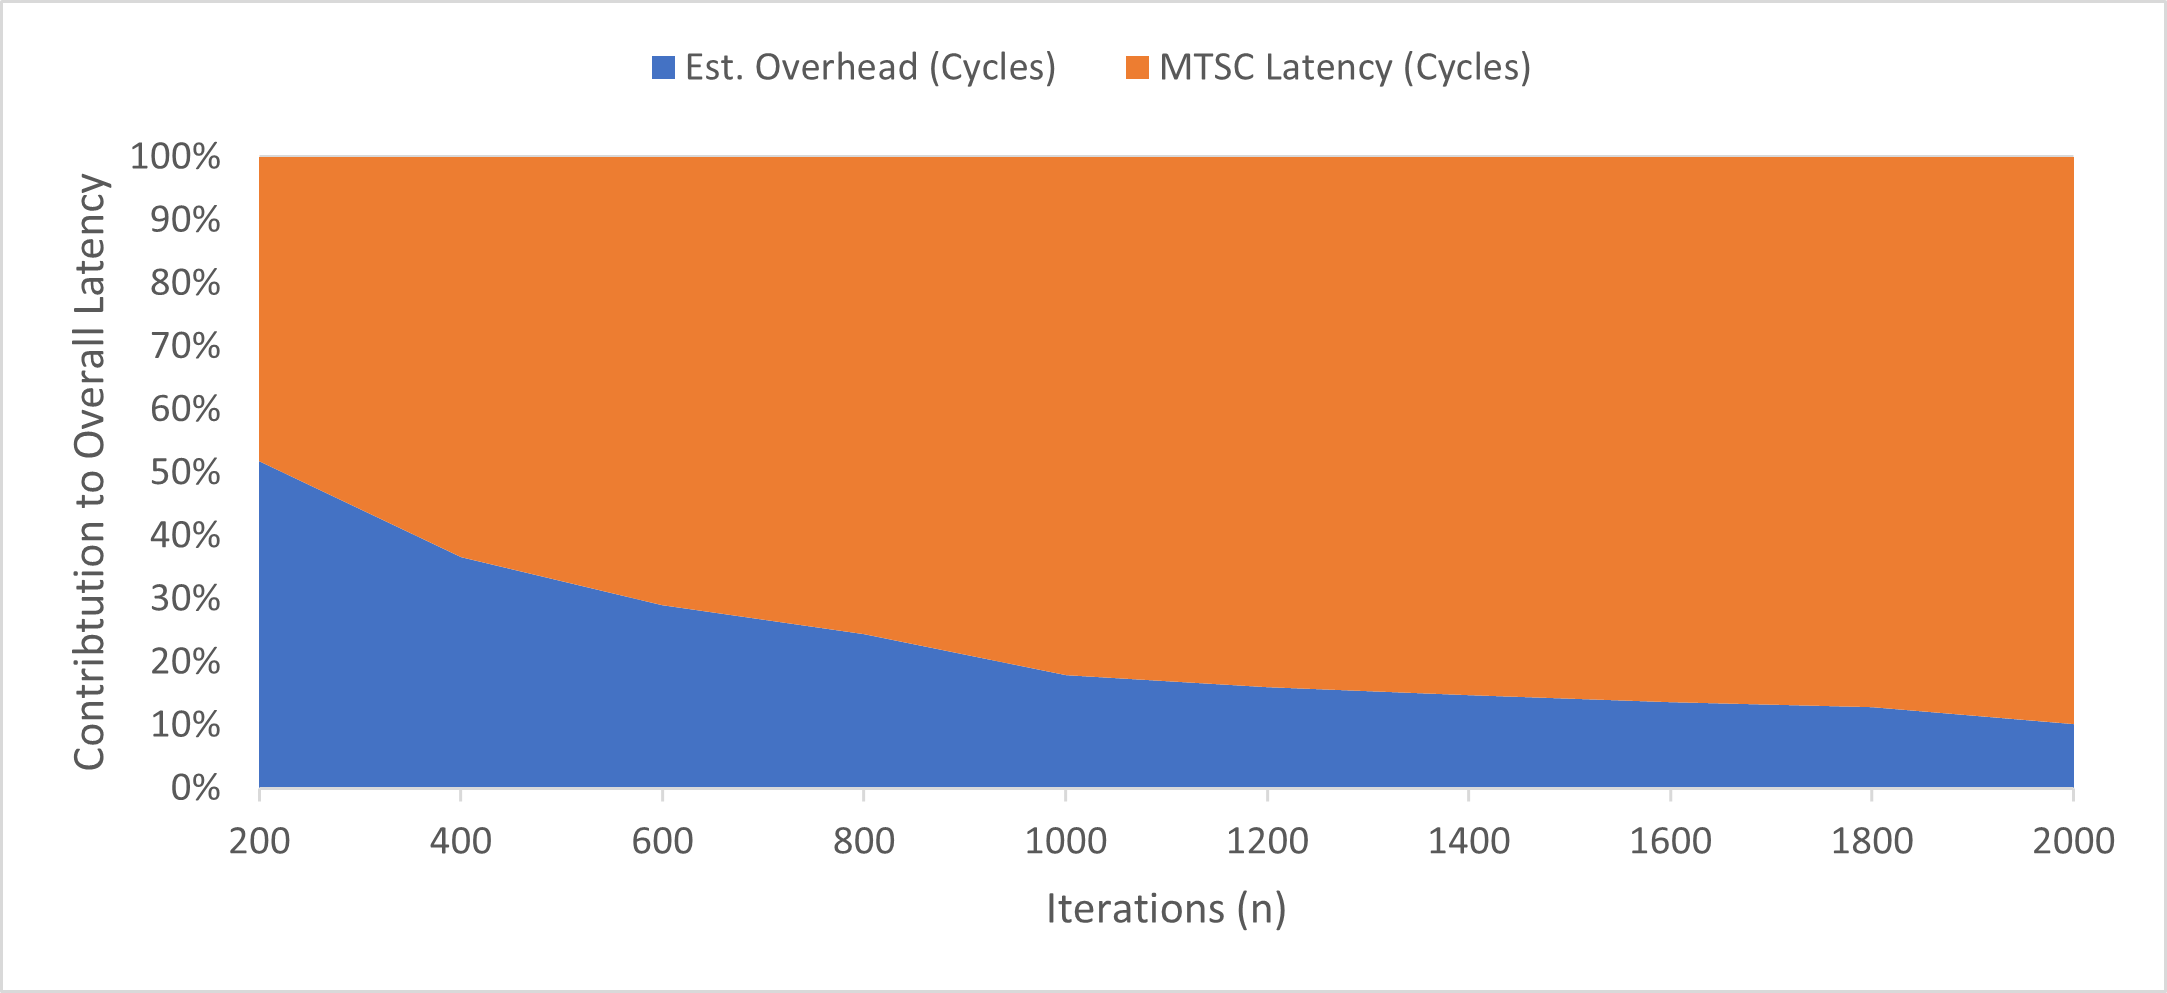
\includegraphics[width=0.9\textwidth]{05_evaluation/images/overhead_percentage.png}
    \caption{Percentage contribution of overhead to total latency}
    \label{fig:overhead_percent}
\end{figure}

\subsection{Conclusions}

Our main conclusion from this investigation is that as we increase the number of iterations the program has to perform, the overhead in the MTMC system contributes less to the overall latency. This claim is supported by \autoref{fig:overhead_percent}, as you can see that with a declining trend in the percentage contribution from the overhead as iterations increases. What we can then conclude is that MTMC systems in which the off-chip function has a large processing latency will perform more equally to their MTSC equivalent systems, therefore, it advised to users of SystemNaim to code their programs in such a way that the designated off-chip function has as much processing time as possible i.e. it has a loop with a large bound within it. If the users fails to do so, they might end up with an MTMC system that performs worse than its STSC counterpart, as can be seen in \autoref{fig:latency_v_iter} when steps = 200. 

Further, by observing the relationship between the latency of the STSC and MTSC system in \autoref{fig:latency_v_iter}, and \autoref{tbl:system_results}, we can see that exploiting the parallelism in the program gave us approximately 48\% reduction in latency, this is due to the fact that there were two sums, $s_1$ and $s_2$, that we calculated in parallel. We can extrapolate from this and say that if you had a program which had three segments which could be run in parallel you would be able to achieve a 3x speed up, and as you increase the number of parallel segments, be they a loop or some other part of the program, you can achieve further performance increases. Therefore, it is advisable to users of SystemNaim to analyse, and potentially rewrite, to exploit as much parallelism as possible while also offloading as much processing to the child as possible.

However, a user must be careful in where they place their off-chip function call. If placed within a loop the overhead does not occur once, but rather it occurs for remote function call. Now this may not be too much of a concern if the processing latency of the off-chip function hardware is high relative to the overhead, but it would be preferable to try and reduce the number of calls to off-chip functions to reduce the contribution the overhead latency makes to the total latency of the system.

From the \autoref{tbl:system_results}, we can see that as we increase the number of iterations the MTMC system approaches the same percentage reduction latency as the MTSC system, compared to the STSC system. This 48\% reduction represents the maximum performance gain we can get from running the program as a multi-FPGA system, and therefore a 42\% reduction, which is what is achieved when we run the system at steps = 2000, proves that SystemNaim is able to create a multi-FPGA system that lets the user achieve a latency decrease without the overhead outweighing the performance gains, which is a major contribution specified in \autoref{sec:contributions}. 

\subsection{Interconnect Latency Variation}

One thing of note, is that the stochastic nature of the interconnect is likely due to the polling issue mentioned in the previous investigation, however as can be seen in \autoref{tbl:system_results}, the overhead tends to be centred around an average value of 1,570 cycles which is close to the overhead measured in \autoref{tbl:spi_clk_results} for the 5MHz SPI clock, the same speed as the SPI clock in this investigation. The range of the measured overheads is 304 cycles, thus, the total overhead latency will be at most 20\% away from the average. This can be seen as an issue for programs with low latencies, but as mentioned above those programs wouldn't be advisable for SystemNaim. 

\subsubsection{Too few resources for MTSC}

A final thing that can be discussed is the necessity for the both the MTSC and MTMC systems to instantiate two hardware modules to calculate $f(x)$. While not the case in this investigation, the hardware module for $f(x)$ may potentially be very resource intensive, specifically, mathematical functions tend to use a lot of DSPs. In the case where a single FPGA may not have enough DSPs, or any other resource, to instantiate two modules to compute $f(x)$, you would no longer be able to create an MTSC system. As an example if each $f(x)$ module took 3 DSPs and our FPGA only had $5$, we would be one short of the required $6$. The user's options would then either be to run the system sequentially, and achieve the results of an STSC system, or it would be to instead use multi-FPGA solution and utilize an MTMC system. Therefore, SystemNaim can solve the issue of a user having FPGA boards with too few resources to implement their design. This would be a real-world motivation for using a multi-FPGA system and thus provides credence to the purpose of SystemNaim.

\section{Usability}
\label{sec:usability}

One of the major motivations of SystemNaim is increasing the accessibility of multi-FPGA systems to people who may not be very hardware proficient. The way we have tried to tackle this goal is by creating a HLS tool which requires knowledge of C90 and basic programming constructs, therefore allowing the tool to be used by a larger group. 

In order to illustrate the usability of the tool we will go through a design example, where we create a multi-FPGA system in SystemNaim,  and then perform a qualitative comparison to creating a similar system but purely in Quartus II using only SystemVerilog and the IP catalog.

\subsection{Design Example: Numerical Integration}
\label{sec:design_example}


For this design example we have decided to show how we implemented the Composite Simpson numerical integration method that was used in the investigation in \autoref{sec:sys_perf}.


\subsubsection{Writing the program.}

The first step for any user would be to write the C code. For this example in particular this took around 15 minutes and the original C code Listing \ref{lst:c_simp_st}. The user must then tell the tool which functions they wish to run in parallel, by encapsulating those functions inside either a “split” or “split\_fpga” block. An example of this is shown in Listings \ref{lst:org_to_par} and \ref{lst:par_to_off}. The case when a user decides to use “split\_fpga” is of the primary focus of this section, therefore, from now on we assume that decision has been taken. \textit{Note: The first function in a “split\_fpga” block is the one that will be run on the child FPGA.} 

Currently, the tool will need to be compiled by the user, however, to make this process easier a Makefile has been provided. \autoref{fig:dir} shows the directory structure for the SystemNaim tool. Running the command “make” while in “Working Directory” will compile the tool.

A test bench folder, “tb”, is also provided. However, this was mainly used for testing during development and most programs created by SystemNaim should not need to be tested. If a user does wish to test their program they will need to install Verilator, and it should be noted that programs which use the “split\_fpga” construct are unable to be tested. Instead, it is recommended to test the same program using the “split” construct instead.

\begin{figure}
\centering
\begin{minipage}{0.47\textwidth}
    \dirtree{%
    .1 Working Directory.
    .2 bin.
    .2 include.
    .2 out.
    .2 hardware\_files.
    .3 parent\_fpga.
    .4 sysNaim\_spi\_handler.sv.
    .4 sysNaim\_master\_mux.sv.
    .4 sysNaim\_instr\_encoder.sv.
    .3 child\_fpga.
    .4 sysNaim\_spi\_slave\_handler.sv.
    .4 sysNaim\_slave\_muxsv.sv.
    .4 sysNaim\_instr\_decoder.sv.
    .3 platform\_designer.
    .4 parent\_cpu.qsys.
    .4 child\_cpu.qsys.
    .2 src.
    .2 tb.
    .2 Makefile.
    }
\end{minipage}
\caption{Current base SystemNaim directory.}
\label{fig:dir}
\end{figure}

Once the code has been properly modified, the user can then pass the program files as argument to the tool, which at this stage is an executable, and in the “out” folder they will find the output Verilog files which describe their program as a set of hardware modules.


\subsubsection{Implementing the system in Quartus.}

The next few parts require the use of Quartus Prime, Intel's Platform Designer and the NIOS II system. Pre-made files are provided for the Platform Designer, so the user isn't required to have an in depth understanding of that tool. However, the ability to assign pins and create a top level file in Quartus will be needed.

The following instructions will also be relatively brief, as they are not intended to be used as a guide but rather to give an overview of the complexity of creating a system. Most of these steps are pretty simple, however they can appear to be complicated to a first time user of Quartus Prime since it is a very bloated and non-self-explanatory tool. 

The first thing a user will need to do is create a Quartus project and select their FPGA. They will then need to create a top level clock and assign names to 4 of the GPIO pins on their FPGA. Any names will work, but we recommend the following: SPI\_MISO, SPI\_MOSI, SPI\_SS, SPI\_CLK. Add these to the top level file, preferably a block design file (shown in \autoref{fig:qp_pins}), and they will be used later.

\begin{figure}[!htb]
    \centering
    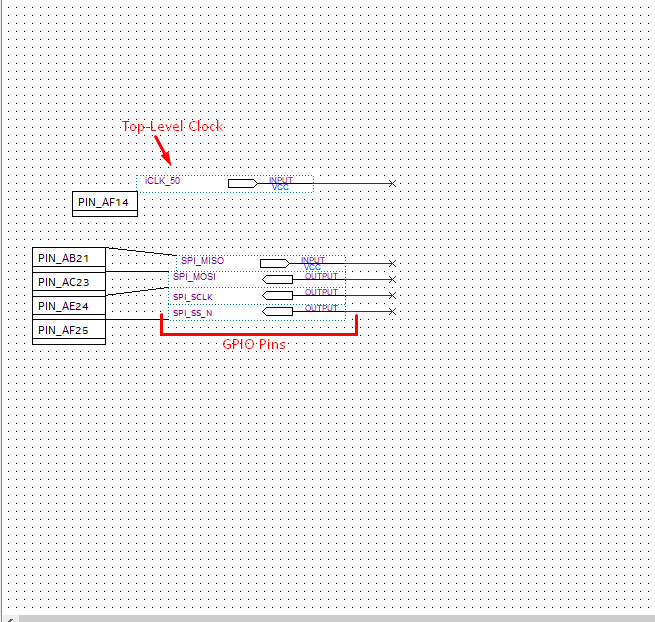
\includegraphics[width=0.9\textwidth]{05_evaluation/images/just_pins.png}
    \caption{Quartus Prime: Top Level BDF w/ GPIO Pins and System Clock }
    \label{fig:qp_pins}
\end{figure}

\subsubsection{Platform Designer}

Now we move onto the Platform Designer. This tool allows you to quickly connect up hardware modules and will allow the user to connect their custom hardware with the NIOS II processor. This processor will act as a controller for our hardware, and will tell it when to start operating as well as provide it the initial inputs. To streamline the process of creating a new NIOS II system, two “.qsys” files have been provided. 

When you open up Platform Designer, you will be prompted to select which “.qsys” file you want to open. These files save the design you have been working for, but also allow us to distribute pre-made systems. Open up the “parent\_cpu.qsys” file, and you should see something similar to \autoref{fig:pd_start}.

\begin{figure}[!htb]
    \centering
    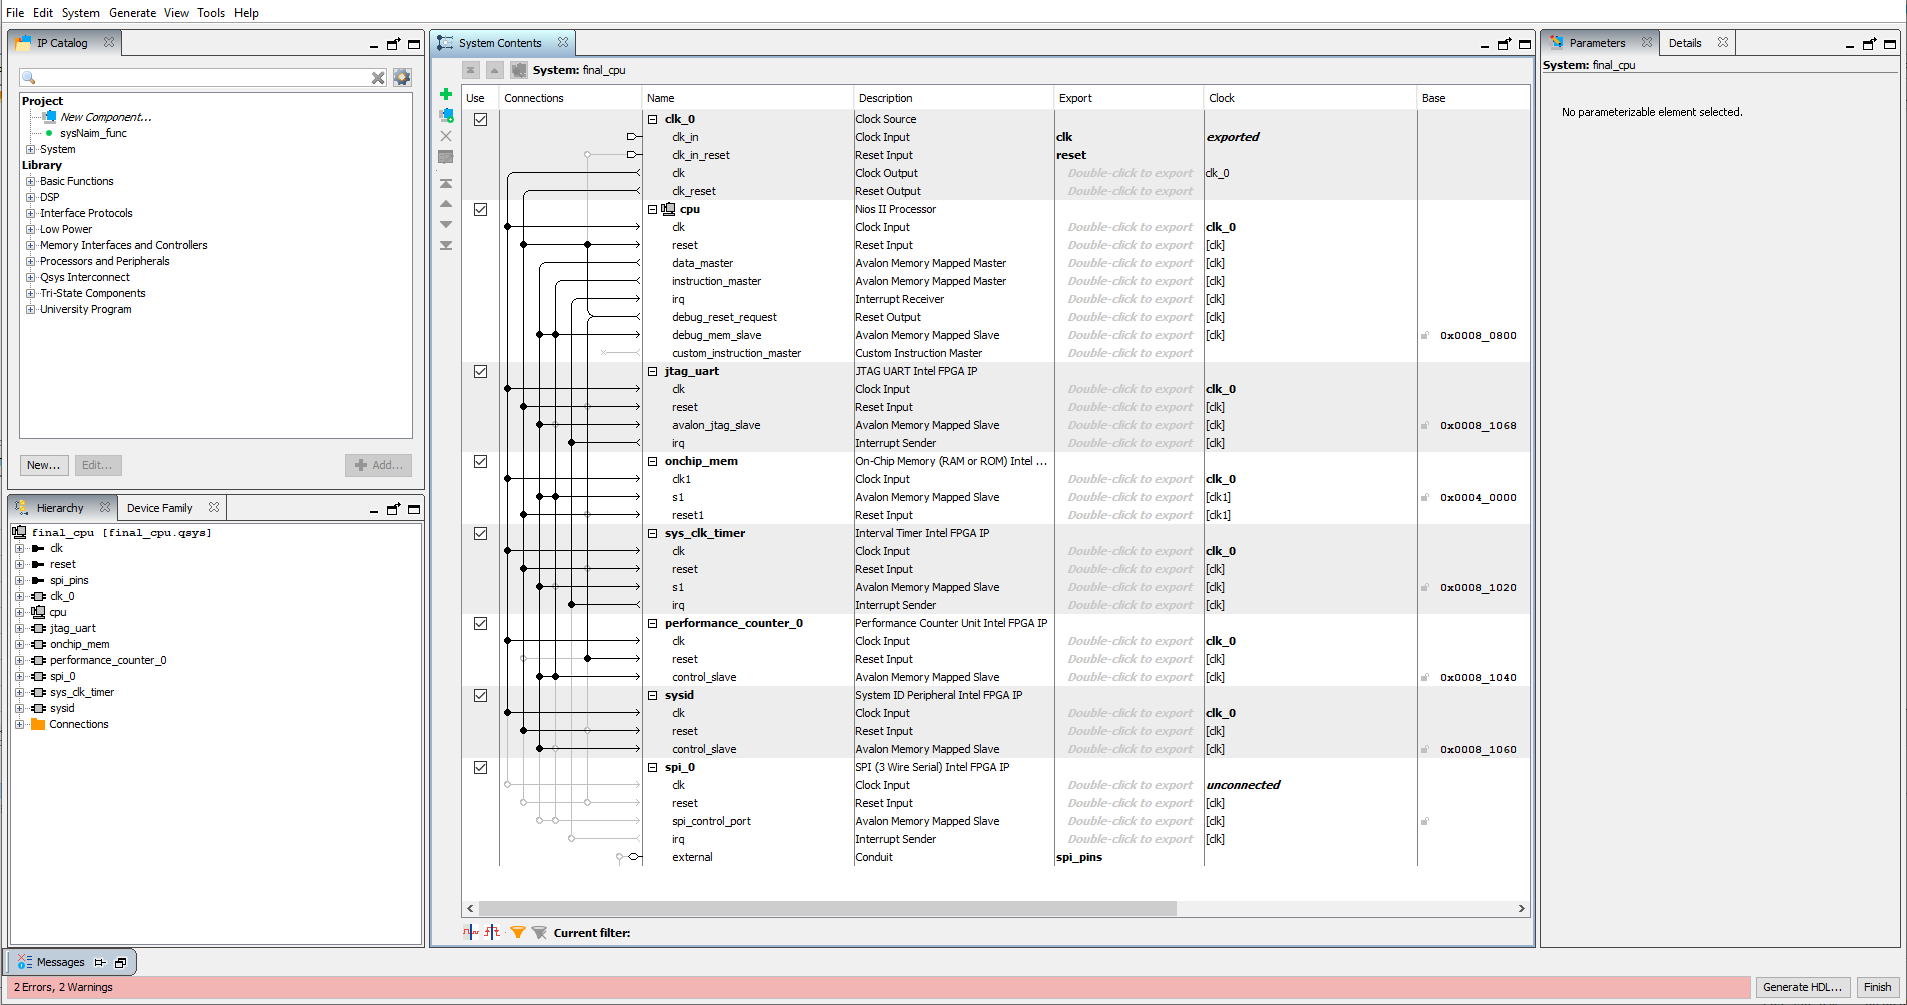
\includegraphics[width=0.9\textwidth]{05_evaluation/images/pd_no_module.png}
    \caption{Platform Designer: System before we add custom hardware.}
    \label{fig:pd_start}
\end{figure}

The user can then add their own custom hardware to the system. In order to do so, they need to click “New...” in the IP Catalog, which results in another window being opened: the Component Editor. In the first tab of this window, “Component Type”, a user can specify the name of their module. More importantly, they need to go to the “Files” tab to include the files generated by SystemNaim. In this tab, they need click “Add File...” under “Synthesis Files” and select all the files generated by SystemNaim in the “out” folder\footnote{It is possible to select only the files needed by the “sysNaim\_host\_top.sv” file, as well as the files needed by its dependencies. But this might get tedious for larger systems.} and then also add the files in the “hardware\_files/parent\_fpga” folder. The user must then find the “sysNaim\_host\_top.sv”, in the file list, and set its attribute to “Top-level file”. 

\begin{figure}[!htb]
    \centering
    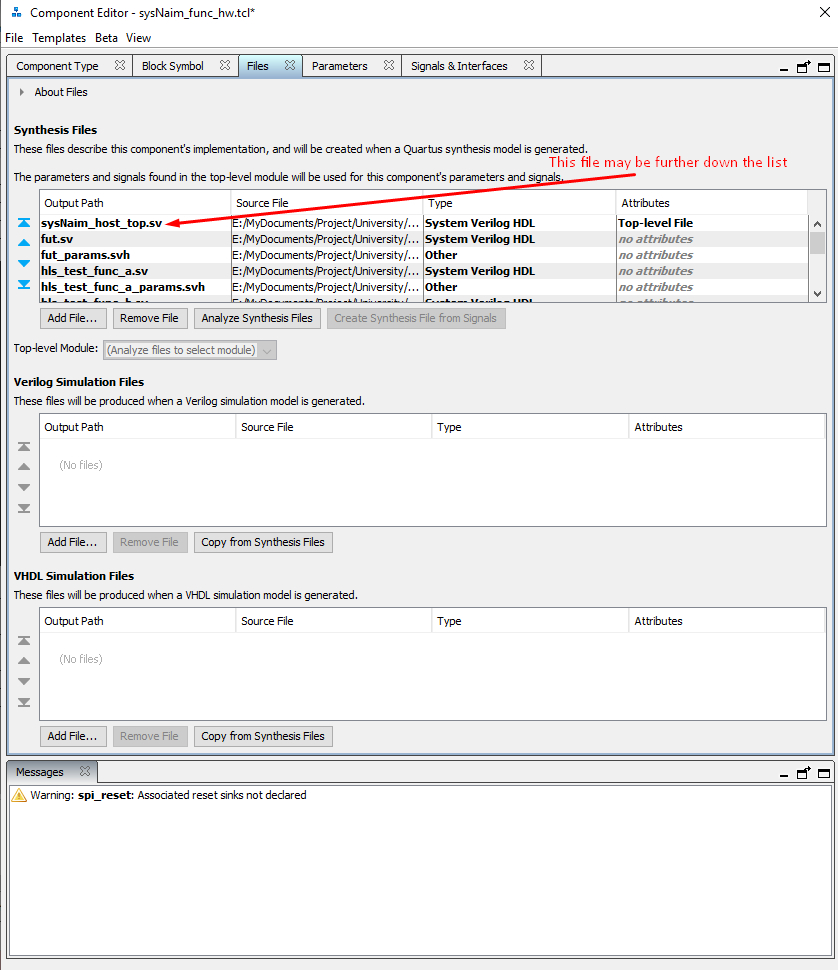
\includegraphics[width=0.9\textwidth]{05_evaluation/images/pd_sys_files.png}
    \caption{Platform Designer: Generated files added to the component editor.}
    \label{fig:pd_files}
\end{figure}

The user can then click “Analyse Synthesis Files”, if this step does not produce any errors they can move onto the “Signals \& Interfaces” tab. This tab will likely be a mess, and it is recommended to delete all pre-existing entries on the left sub-window. The user will then need to add the interfaces and signals until it looks like \autoref{fig:pd_interfaces}. The user should take extra note of the text in grey next to each signal and interface as this denotes type and is extremely important to get correct for proper synthesis.

\begin{figure}[!htb]
    \centering
    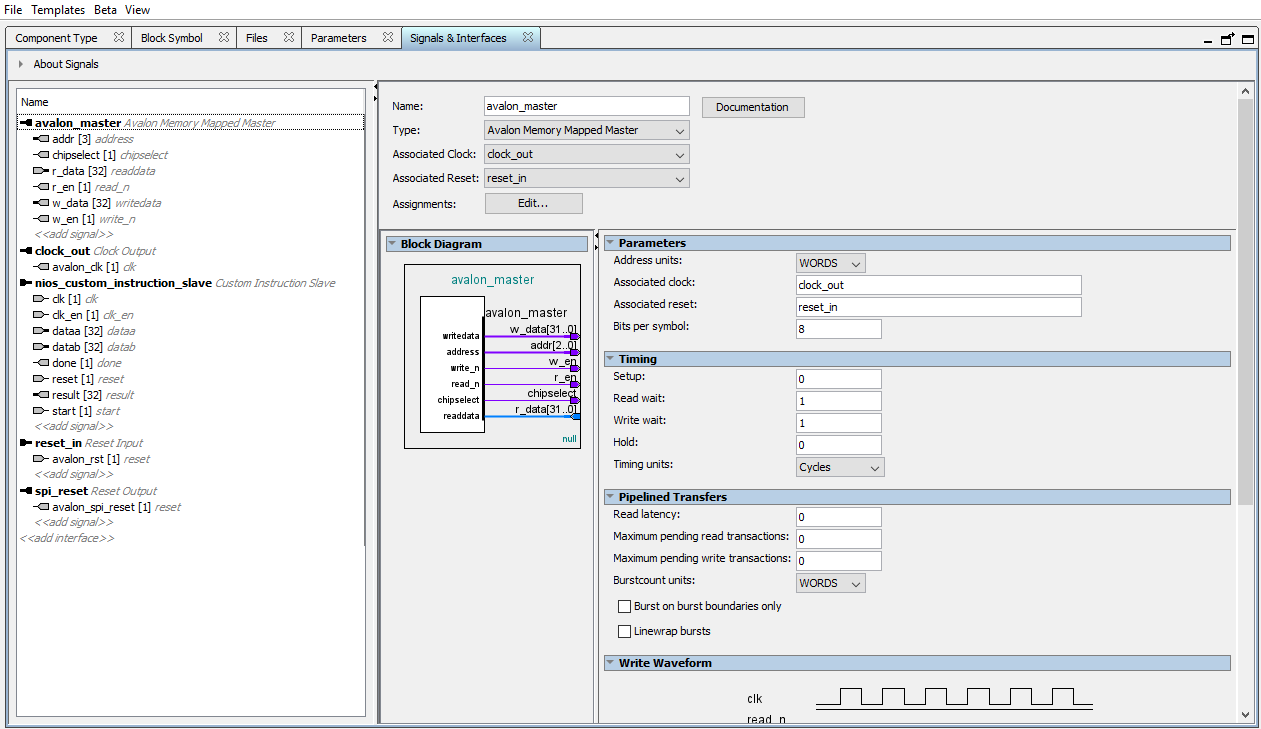
\includegraphics[width=1\textwidth]{05_evaluation/images/pd_interfaces.png}
    \caption{Platform Designer: Complete interface \& signal list for the custom hardware}
    \label{fig:pd_interfaces}
\end{figure}

Once all the signal are added, the user will need to click on the “avalon\_master” interface and set the “Address Units” to “WORDS” and the “Write wait” to “1”, shown in \autoref{fig:pd_avalon}. They will also need to select the “clock\_out” interface and set the “Clock rate” to “50000000” and enable “Clock rate known”, refer to \autoref{fig:pd_clock}.

\begin{figure}[!htb]
    \centering
    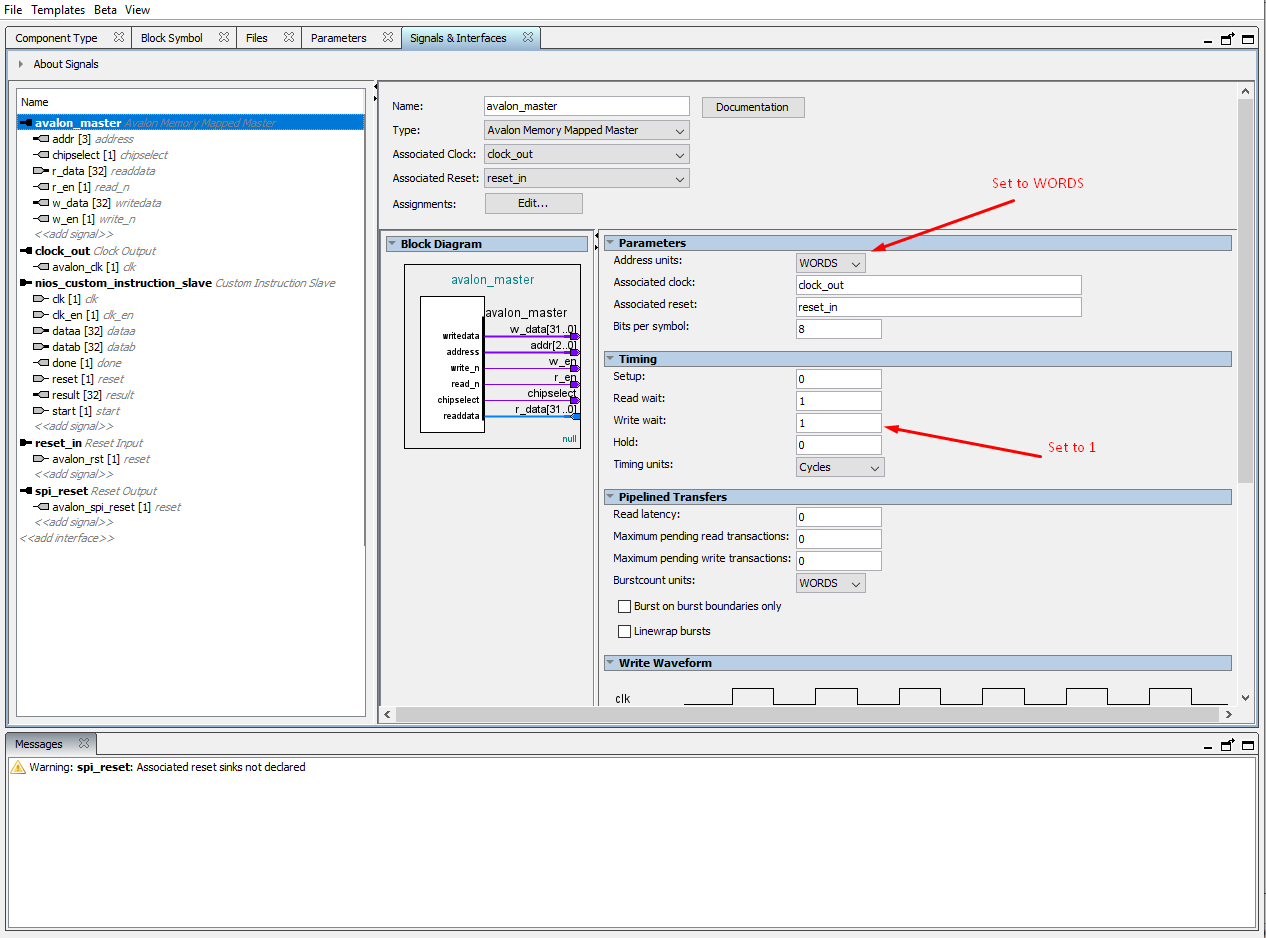
\includegraphics[width=1\textwidth]{05_evaluation/images/pd_avalon_config.png}
    \caption{Platform Designer: Avalon config}
    \label{fig:pd_avalon}
\end{figure}


\begin{figure}[!htb]
    \centering
    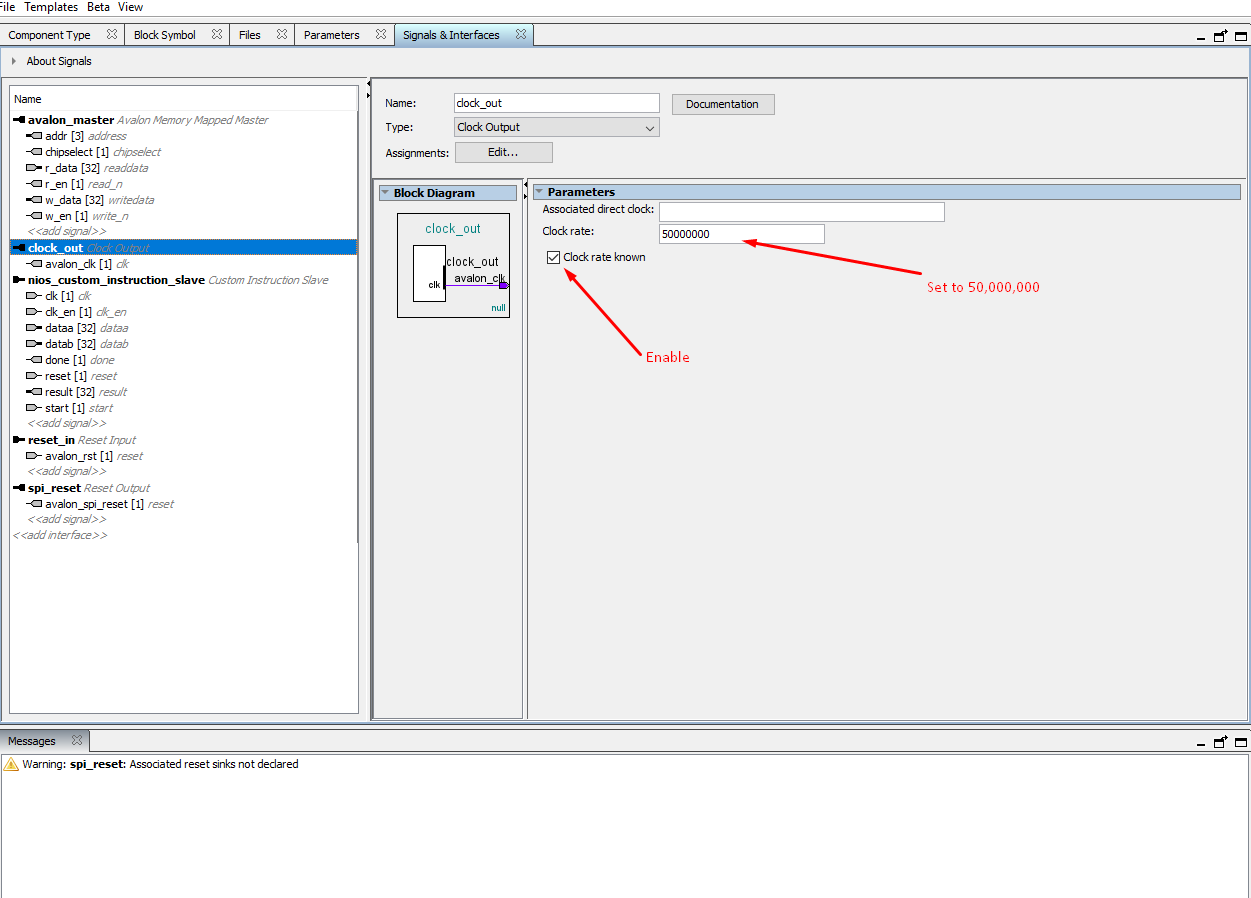
\includegraphics[width=0.9\textwidth]{05_evaluation/images/pd_clock.png}
    \caption{Platform Designer: Clock output config}
    \label{fig:pd_clock}
\end{figure}

A user may then click “Finish...” to save their design and exit out of the “Component Editor”. Now that their module has been added to the catalog, a user can search for their custom hardware and add it to their system. Once their module has been added, they will need to connect it to the other modules in the system. The important modules are “CPU” and “spi\_0”. The first represents the NIOS II processor, and we connect it to our module through the Custom Instruction” interface. The “spi\_0” is an IP core provided by intel to interface with an SPI channel. This module will be driving the GPIO pins, while the user's custom hardware will be controlling it and providing it data.

To connect the custom hardware module, click on the dots shown in \autoref{fig:pd_connections}. They should be empty white circles initially, and then should fill when enabled. The user should then save the system and click “Generate HDL”. In the prompt that shows up, most default settings should be kept however the user should make sure “Create block symbol file (.bsf)” is enabled. “Generate” can then be clicked and in the “Platform Designer” window the user can press “Finish” to exit the tool.

\begin{figure}[!htb]
    \centering
    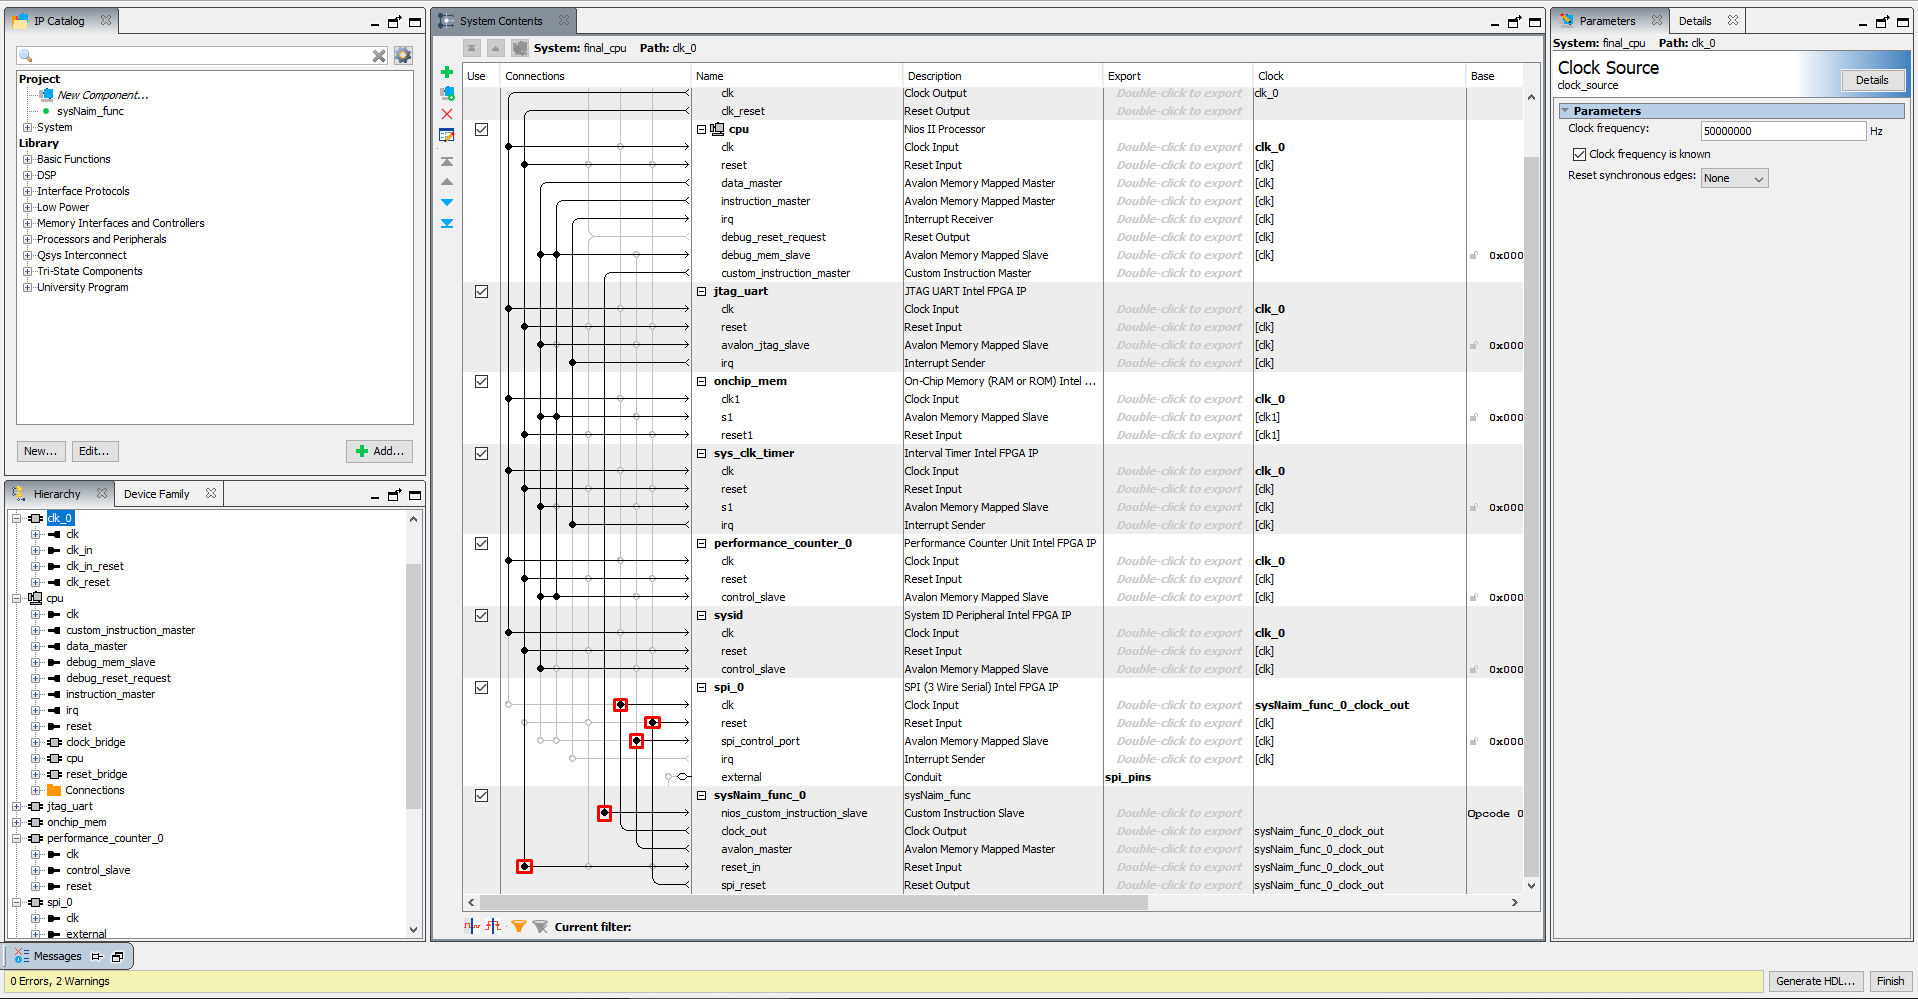
\includegraphics[width=0.9\textwidth]{05_evaluation/images/pd_connections.png}
    \caption{Platform Designer: Connections to the custom hardware}
    \label{fig:pd_connections}
\end{figure}

\subsubsection{Back to Quartus}

Once back in Quartus, the user will need to add the “parent\_cpu.qsys” file to the project files. They can then add their system, which will be named “parent\_cpu”, to the top-level file containing the pins. Wire up the pins to their appropriate ports on the CPU module, as shown in \autoref{fig:qp_connected}. Then add a VCC block and connect it to the “reset\_n” port. The user may then synthesize the top-level file and load it onto the FPGA.

\begin{figure}[!htb]
    \centering
    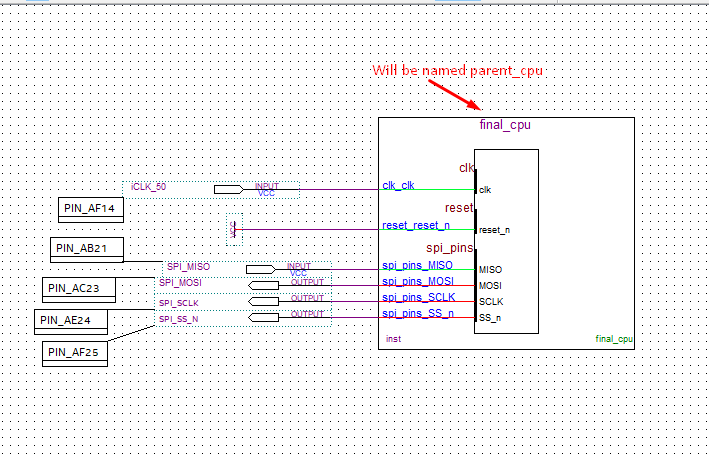
\includegraphics[width=0.9\textwidth]{05_evaluation/images/qs_cpu_connected.png}
    \caption{Quartus Prime: NIOS System connected to pins in top-level file.}
    \label{fig:qp_connected}
\end{figure}

\subsubsection{NIOS II Eclipse}

The final tool the user will need to use is the NIOS II Software Build Tools for Eclipse. It is recommended that the user read the following: pages 4-7 of “My First NIOS II Software” \cite{nios-ii-first-prog} and chapter 3 of “NIOS II Custom Instruction User Guide” \cite{nios-ii-inst-guide}.

Once the user understands how to create a NIOS II project and call custom instructions they can run their own custom hardware on their FPGA.

Example code files for both the child and parent FPGA can be found in Listings \ref{lst:parent_code} and \ref{lst:parent_code} respectively.

\subsubsection{Child FPGA Setup}

The sections starting from opening up Quartus will need to be repeated in order to set up the user's child FPGA. When performing these steps again most are the same, except when in the “Platform Designer”, the user should open up the “child\_cpu.qsys” file instead. They must also set the “sysNaim\_remote\_top.sv” as the top-level file, and include the hardware files in the “child\_fpga” folder instead of the “parent\_fpga” folder. Calling the function in NIOS II for Eclipse will be the same except that the function name will be different.

\subsubsection{Running the System}

Before the bitstreams are downloaded onto the FPGAs, the user should first connect the GPIO pins they assigned names to. So the SPI\_MISO pin on the parent FPGA should be connected to the SPI\_MISO pin on the child FPGA, and so on for all the other SPI pins. One this is done the FPGAs can be programmed, ready for the systems to be run.

To run the system, the child FPGA starts first so that it is ready to receive a transaction from the parent FPGA. Once the child FPGA has been started, the parent FPGA can be run. When the NIOS II terminal displays the result, the system has completed operation.

\subsection{Creating a Multi-FPGA System from Scratch}
\label{sec:scratch}

Going through a step-by-step design example for implementing a multi-FPGA system would likely take an obscene amount of pages and would do very little to showcase the main differences in complexity between such a system and one implemented using SystemNaim. Instead, the following sections will provide an overview of the main challenges and considerations that one would have to think about if they were to create a system just using Quartus Prime and SystemVerilog.

Afterwards, a comparison will be made of performing the same task using SystemNaim. Both the benefits and disadvantages for both solutions will be given to provide a fair and a balanced evaluation.

\subsection{Computing the Result.}
\label{sec:dedicated_hardware_computation}

The first task a user would have to complete is designing the system which computes their desired function. Unlike programming in software, designing in hardware requires a full understanding of the system before any HDL is written.

As an example, let us consider a module which computes the value for a function, $f(x)$. A user must consider design decisions such as, is this module combinational or sequential? Is a ready signal necessary to tell a connected module whether this module is ready to take in data? Will I assume all modules connected to this one know the latency of this module, or will there be a done signal?

Before the computation within the module is reasoned about, a user must decide how this module will be used by the hardware blocks connected to it. The interfaces of a module are of key importance since they determine how a module accepts data and how it should output data once it has finished computation.

Even when we can start writing the hardware logic, the paradigm shift from software programming becomes larger. For loops don't necessarily exist in Verilog the same way as normal programming languages. To implement something similar a state machine, whose computation resembles a for loop written in assembly, must be designed. However, this may not be the most optimal solution, and instead, having a FIFO as an interface input and grabbing data from it when it is available would be a better way of iterating over data. The latter solution is something very few people, outside those with experience in concurrent programming and queues, would think to implement, but it would result in a more streamlined system with less overhead states.

In comparison to software programming, hardware design requires a user to put much more thought into how the modules connect rather than just what their computations consists. A single mistake in deciding which cycle to pass data from one module to another can cause a cascade of failures, resulting in the entire system being rendered useless. Even debugging is more difficult, you can't merely call your main function with some inputs and print to console in places you think the program is broken. Instead, you have to simulate your entire design, including manually creating valid transactions for you top level module, and then find the issue by following incorrect wire or register values to their source.

\subsubsection{Comparison to SystemNaim}

When creating a system in SystemNaim, it's exactly the same as developing software. You can write a program in C and trust that the tool will create the correct hardware which computes the same result. The main draw of HLS is that a user no longer needs to worry about timing violations or what number states are necessary for this module, instead they can focus on the actual computation which the system needs to implement. Creating dedicated hardware to compute the Composite Simpson numerical integration would likely take a few hours, but in SystemNaim it only takes 15 minutes. This speed-up in development time is crucial for implementing larger systems in hardware within a reasonable time frame and is one of the major contributions we say SystemNaim achieves in \autoref{sec:contributions}.

However, the increase in user productivity does come at cost. The output Verilog will likely have much worse latency than hardware designed for a specific system. If an individual were to create dedicated hardware to compute the Composite Simpson numerical integration, the latency would be much lower than the system created in SystemNaim. Therefore, a user must decide if the increase in latency of the resulting hardware is worth the reduction in development times. For larger systems this potentially may be the case as it would be otherwise unfeasible to create all the hardware manually.

\subsection{Converting to Multi-FPGA}

The main purpose of SystemNaim is to streamline the process of creating a multi-FPGA system. But, what issues and challenges would one face if they decided to create a multi-FPGA system using only Quartus and Verilog. Firstly they would have to decide how the two FPGAs would communicate with each other. Usually this is done over a communication channel such as SPI which then begs the question: whether they would want to use Intel's SPI core, or any other communication IP core, to control their channel or create their own hardware. The latter is ill-advised unless they wish to create their own protocol, but the former usually requires an understanding of an Intel designed interface.

In the case of the Intel SPI core, there is an Avalon-MM interface, which requires the user to control signals such as: address, read data, write data, read/write enable, and chipselect. All signals have their own purpose and misunderstanding any of their uses leads to an inability to interact with the core. Therefore, in order to use one of these cores a user has to design a hardware module which correctly interfaces with the core so that they are able to send and receive data over the channel. Sometimes, the provided core on the child FPGA may have a slightly different implementation, which requires an additional hardware module to be created in order to interface with it correctly.

But once the required interfacing hardware is created, the user must then decide what data they wish to send over. Sending more data over the channel allows for more processing to occur on the child FPGA, however this incurs a latency cost as explored in \autoref{sec:interconnect} and thus sending too much data will slow down the system. On the other hand, sending too little data will reduce the amount of processing that can be done on the child FPGA as it won't have anything to actually process. Potentially, the designer could only use the communication channel to send commands to the off-chip and not any actual data. This would mean that all data would need to created on the child FPGA, or known by it at compile time, thus drastically reducing its versatility at run-time. Using the Composite Simpson example once again, the designer could decider that the values of $a$, $b$, $n$, and $h$ are never going to change and thus no data needs to be sent to the child FPGA when it's computing its sum. However, this would mean that if the user wanted to integrate over a different part of the function they would need to recompile the entire system. 

The resulting decision ends up being a balance between being able to compute as much as possible on the child FPGA and not incurring too much of latency cost from using the communication channel, but a user can tailor it to their specific needs.

The next issue the user faces is connecting this communication channel to their main system. Assuming they have decided what data is being sent over and what processing is occuring on the child-FPGA they will then need to create a new data path to send the correct data to the communication channel. They will then need to decide if they want to wait for the processing off-chip to be finished before they continue any other operation or if they would like to perform some computation on the parent FPGA in parallel. The latter is strongly advised, but requires additional hardware to wait for both data paths to finish processing.

If the system has already been designed with parallelism in mind, and the user wished to offload one of the parallel data paths to the child-FPGA, then the new data path will likely just be a modification of a pre-existing one. If the system had no parallelism beforehand, then creating a new data path may require an entire overhaul.

Overall, creating a multi-FPGA system is not just about setting up a communication channel but rather considering which parts of the system would benefit from being processed off chip, and what data those parts require. But it is still a tedious and long process to create a functioning communication channel.

\subsubsection{Comparison to SystemNaim}

In SystemNaim, we use function calls as a method of allowing the user to decide what processing occurs off and on-chip. This makes it much easier for new users to split their program across multiple FPGAs, which is a requirement of the HLS tool specified in \autoref{sec:hls_design}. They don't have to worry about interfacing correctly with the SPI core, or creating a new data path to accommodate for the off-chip processing. Instead, they can treat it as a normal function call and nothing more. Of course, following from \autoref{sec:sys_perf}, there are recommendations that the user should follow when creating their program, but they are free to explore designs as they wish, and they can experiment with choosing which parts of their program to process off-chip without having to go through the hassle of re-hauling their entire system, if they had chosen to do it manually.

It goes without saying, though I will say it, that there aren't only advantages to using SystemNaim. The user is limited to only being able to design functions with two inputs, which does limit the potential use cases. If they had designed their own hardware system, they would be able to transmit as much data as possible. SystemNaim also forces each transaction across the channel to be 32 bits long, in order to ensure a full integer can be sent across. However, some systems may not need to full 32 bits which results in unneeded additional latency.

Once again, the decision to use SystemNaim or not is a balance between latency and development time. A manually designed system, focusing on one application, will be faster and will use less resources. But, it may take much longer to create. When creating SystemNaim it took us a week to create the hardware to control communication channel and even longer to debug it. Therefore, I would posit, that even though it may result in latency increases, the time saved from using SystemNaim, and any HLS tool derived from it, will allow for much larger systems to be created and for more experimentation on multi-FPGA platforms to take place.

\subsection{Conclusion}

The sections above show that while SystemNaim does create less optimized systems, than dedicated hardware, it does streamline the development process and reduce the time taken to get a system running, which is one of the primary contributions mentioned in \autoref{sec:contributions}. To further illustrate this two example project timelines are shown in Tables \ref{tbl:time_sysNaim} and \ref{tbl:time_custom}. As a disclaimer, these values have been chosen from my own experience, they may vary from person to person, and external factors may also affect, for example if the FPGA had a hardware defect and extra time was spent debugging that. The durations stated in \autoref{tbl:time_sysNaim}, assume the user is following the design example above for the first time, and have no knowledge of their FPGA's pin layout. The overhead times can decrease greatly as the user becomes more proficient in these tools, leaving only the development as the main contributing factor. \autoref{tbl:time_custom} assumes the individual implementing the system has an amount of experience with hardware development close to ours, as the time values are an estimate of how long it would take us to implement these parts. We also have assumed that the system design already accounts for off-chip processing, and no overhaul is required when reaching the implementation of the channel starts. Finally, it should be noted that a large part of the time spent is mostly in design and debugging rather than the writing of HDL.

From these tables we can see that SystemNaim would save a designer, days in development time and this would be for a relatively simple system. Larger systems take even longer to design in Verilog and Quartus, but the increase in time for SystemNaim or other HLS tools would be far less. Therefore, with some leniency, it can be concluded that we have proved our 3rd contributions specified in \autoref{sec:contributions}.


\begin{table}[]
\begin{tabular}{l|l|l}
Task                                 & Time Spent & Cumulative Time Spent \\ \hline
Programming System                   & 1h         & 1h                    \\
Creating System in Platform Designer & 30m        & 1h 30m                \\
Assigning Pins in Quartus            & 1h         & 2h 30m                \\
Setting up NIOS II environment       & 1h         & 3h 30m               
\end{tabular}
\caption{Time to taken to create a multi-FPGA system in SystemNaim, assuming beginner FPGA knowledge.}
\label{tbl:time_sysNaim}
\end{table}


\begin{table}[]
\begin{tabular}{l|l|l}
Task                               & Time Spent & Cumulative Time Spent \\ \hline
Implementing Computational System  & 3d         & 3d                    \\
Implementing Communication Channel & 3d         & 6d                    \\
Overhead using tools               & 2h         & 6d 2h                
\end{tabular}
\caption{Time to taken to create a multi-FPGA system in with just Verilog and Quartus, assuming intermediate FPGA knowledge.}
\label{tbl:time_custom}
\end{table}


One last note that is important to this analysis, regards to the steps shown in \autoref{sec:design_example}. Many of the steps shown when setting up a SystemNaim system are not related to the development of the program, but rather they illustrate the overhead that comes with getting it to run. Tasks such as; finding a way to control the system, connecting the program hardware to the SPI core, assigning pins to use as the communication channels, would still be present if a user decided to implement their own system from scratch. Potentially the steps regarding NIOS II could be avoided, but then additional effort would be needed to find a way of controlling and testing the system. In addition, pre-made files which streamline these tasks would also not be available and the designer would have to gain a deeper understanding of all the aforementioned tools to complete their system. Therefore, SystemNaim can be said to not only quicken the development process but also the process of getting the system actually running on an FPGA.








    \chapter{Future Work}

Given that SystemNaim was a final year project, and as such we could only put about 9 months of time into it, there are a lot of features that we would have like to have added or expanded upon. This section will go through some higher priority additions that weren't able to be made due to time constraints, but if added would make SystemNaim into a more complete and useful tool.

\section{Actual 'Multi'-FPGA System}

Currently, SystemNaim only allows for two FPGAs to communicate, one parent and one child. Allowing for more FPGAs to be used in tandem would give users the ability to exploit more parallelism within their programs, however it would also come with additional difficulties. The first challenge would be adding an addressing system so that each child FPGA could be identified. It would be likely that the system would just expand, with each child FPGA holding a collection of functions that could be called upon by the parent FPGA when required by the program. The parent FPGA would need to be able to, not only choose the correct function opcode, but also the correct address so that it could call the off-chip function it required. 

This could be added to the remote modules, which are instantiated on the parent FPGA, with each being configured at runtime to signal which child FPGA contains their function. The interconnect would then need to signal to the channel which child FPGA to deliver this command and opcodes to. With SPI this is pretty straightforward, every child FPGA would be connected to the same MISO and MOSI channel and  each would have their own SS\_EN (Slave Select Enable) signal, which would be asserted, by the parent FPGA, when that child FPGA was receiving a transaction. In the case of multiple off-chip functions being called at the same time, there would have to be a queue and the parent FPGA would call each function sequentially. Once it had finished calling all the necessary off-chip functions, it would then need to poll each of the activated child FPGAs, until their processing was complete, to return the result.

The polling, in this case, would likely be done in a round-robin fashion. With each child FPGA being sent a polling transaction, as described in IMPLEMENTATION SECTION, in order until all results had been returned. This does have the potential of causing latency spikes for the entire system. As was explored in \autoref{sec:interconnect}, missing a polling transaction can result in a large amount of additional latency, especially at low SPI Clock speeds, and adding multiple child FPGAs the parent needs to poll can only increase the worst case of a child FPGA missing a polling transaction. The solution for this would be to either know the latency of the off-chip functions, and only poll that child FPGA when it is assumed to have finished computation, or switch to a communication channel where both parties can start a transaction, such as Ethernet.

\subsection{Ethernet}

An Ethernet communication channel would allow child FPGAs to return data to the parent FPGA without the need for constant polling. Furthermore, only one port is required per device, with this never increasing as the system grows larger, and Ethernet can operate at a higher channel bandwidth than SPI thus further reducing the total overhead latency. The downside comes from the added complexity required in SystemNaim's custom hardware. Ethernet requires each device to be identified by a 48-bit number(MAC address) which cannot be assumed to known at runtime, therefore the parent FPGA would initially need to broadcast a request to all child FPGAs, for them to send an Ethernet packet containing their MAC address. As the parent FPGA receives these packets, they would need to store them in a lookup table to be able to communicate later on with the child FPGAs.

The additional effort required to get an Ethernet communication channel working would be worth-while as the added channel bandwidth plus capability for larger systems, could allow SystemNaim to implement more latency critical programs as well expand the scope to, in the future, allowing computation on the cloud.

\subsection{Changes to the HLS}

When allowing for systems with 3+ FPGAs a decision has to be made as to whether the user should decide which off-chip functions go on which child FPGA. The essence of SystemNaim is to give the user as much control over the end product as possible and merely remove the tedious hardware development aspects, and thus we'd likely incorporate a method that allowed the user to choose which functions are called on which FPGAs. An example of how this is possible is shown in \autoref{fig:multi_fgpa_hls}. Inspiration was drawn from the C++ STL, with the number between the “<>” symbol representing which child FPGA the function would be placed on (0 could mean the function should be run on the parent FPGA). Off all the challenges that would likely be faced when implementing this addition, the modification to the software side is probably the least difficult in a technical sense, however, the final decision on its implementation will define how users interact with this aspect of the system, and thus it is worth conducting a design investigation if there are any plans to ever add this feature in the future.

\begin{figure}[!h]
    \centering
    \begin{minipage}{0.5\textwidth}
    \begin{minted}{c}
split_fpga{
    holda = <0>hls_test_func_a(h, n);
    holdb = <1>hls_test_func_b(h, n);
    holdc = <2>hls_test_func_c(h, n);
    holdd = <3>hls_test_func_d(h, n);
}
    \end{minted}     
    \end{minipage}
    \caption{Method of allowing user to dictate which child FPGA a function is called on}
    \label{fig:multi_fgpa_hls}
\end{figure}

\section{General HLS Optimizations \& Additions}

\begin{itemize}
    \item Adding pipelining, FIFO's, arrays and maybe even giving the user access to FPGA pins
    \item Maybe even the off-chip function can start to use FPGA pins
\end{itemize}

As discussed in \autoref{sec:usability} the main downside of SystemNaim is the increase in latency of the hardware it produces, and as explained in DESIGN SECTION the decision to not spend too much time on creating optimal hardware was an intentional one. However, if SystemNaim were to be improved on in the future, optimizing the HDL generated by the HLS would make it much more appealing when compared to creating a dedicated hardware system. Below is a list of different optimizations and additions that could be made to SystemNaim's HLS aspect so that a user could create lower latency or more complex systems.

\subsection{Loop Pipelining}

Pipelining is an example of an optimization that would drastically reduce the latency of any loop-based function. In essence, pipelining allows for multiple iterations of a loop to be computed at the same time and is especially useful when a single iteration may take many cycles. However, in order to implement this feature correctly SystemNaim would need to be able to detect data dependencies both within an iteration and between iterations, and thus an extra step of analysis in the tool would need to be added. 

To illustrate the benefit of loop pipelining, a small example will be looked at. Imagine if we had a loop with 100 iterations and each iteration took 5 cycles. To compute this loop fully would require 500 cycles, with no pipelining. To calculate the latency of this loop with pipelining we need to use the formula found in \autoref{eqn:pipelining}. Initiation interval (II), a term that we haven't used yet, is a defined as the number of cycles between the start of each iteration of the loop. For an unpipelined loop the II is equal to the latency of each iteration. If we were to have an II of 1, the best case, the example loop would only take 104 cycles to compute, thus giving a large reduction in latency. With how prevalent loops are in modern programming, adding this feature would benefit a lot of programs that may be implemented using SystemNaim, but would require an overhaul of the line-to-state model currently in use in order to allow for concurrent hardware.

\begin{equation}
    L_{tot} = L_s + I * (N - 1) \label{eqn:pipelining} 
\end{equation}
where:
\begin{conditions}
L_{tot}    &  is the total latency of the loop \\
I    & is the Initiation Interval(Throughput) \\
N & is the total number of iterations in the loop \\
L_s & is the latency of a single iteration
\end{conditions}


\subsection{FIFO's \& arrays}

In \autoref{sec:dedicated_hardware_computation}, a case when a FIFO would be optimal instead of a loop was given. FIFO's have a lot of uses in hardware design, especially when it comes to acting as the middle man between data-producing and data-consuming hardware modules. They can allow for multiple pipelined loops to act concurrently, without consuming a large amount of resources, and can act as queues for feeding data into a function. Giving access to this hardware construct to users of SystemNaim would allow them to create more complex and optimal systems. This would be the same with arrays, which allow for more complex algorithms to be implemented in SystemNaim. 

Being able to store data is of vital important when creating a modern system, however, when deciding what features SystemNaim needed to implement to prove our aims we realized arrays weren't necessary. Nevertheless, in the future adding both of these constructs would vastly increase the versatility of SystemNaim, but not without their share of challenges. For arrays, multiple sources accessing the same part of memory would require multiplexers so that there wouldn't be any contention, which poses the risk of increasing the latency of each access. In terms of FIFO's, the challenge is more on the HLS side. Giving access to all aspects of the FIFO to the user would be tricky without using a class-based method inspired by C++'s OOP. This would result in potentially too large of a change in syntax, and at that point, instead of making changes to the base C language, it would be worth switching SystemNaim's base language to C++. The additional work while large, could open up more possibilities for different hardware modules to be added in the future, with member functions being the designated way of controlling and interfacing with them.

Each addition would require a large amount of work but definitely has merits, and what would be achievable within SystemNaim after they had been added would be very interesting to investigate

\subsection{FPGA Pins}

The final addition that we believe SystemNaim would benefit from, is the ability for users to access FPGA pins from their top-level function. Pins on an FPGA are use as I/O and allow for external data streams to be processed on the FPGA. They are essential for most real world FPGA use cases, and giving users the ability to interface with external devices would make SystemNaim a more versatile tool. Users would be able to stream in data from an Ethernet or USB port and user their multi-FPGA system as an accelerator within a larger system. 

Instead of giving access directly to the pins themselves, which would breach the software vs hardware programming paradigm and would defeat the purpose of an HLS tool, we could allow for FIFO's to be implemented at the top-level and then expect the user to develop some hardware to get the data from their external source into said FIFO. This would, of course, require some hardware proficiency on the user's behalf, but it would still give increase the use case of SystemNaim. It would be of interest to actually perform an investigation into the possibility of requiring no hardware proficiency from a user, but still giving them access to I/O pins and ports within the HLS tool.

Another benefit of such a feature would be for child FPGAs to also be able to access their own I/O pins, and thus would be able to consume data from their own sources rather than being given it by the parent FPGA. From \autoref{sec:interconnect}, we know that this would reduce the transfer overhead if we no longer need to send data operands across the channel, therefore, further reducing the latency of the total system.

\section{Inter-FPGA Data Streaming}

\begin{itemize}
    \item Potentially you could stream data through the channel in order to get more than two operands across.
    \item You could also split the channel into two. One for starting off-chip functions and one for streaming data between the FPGAs.
\end{itemize}

    \chapter{Conclusion}

To summarize the results of our investigation we will revisit the contributions and aims that were originally outlined in \autoref{sec:intro}. The contributions were as follows:

\begin{itemize}
    \item \textbf{Proved it is possible to automate the process of creating a multi-FPGA system.} \autoref{chp:eval} shows SystemNaim working in 2 different testcases, and \autoref{sec:full_system} shows the design flow when using the tool. As shown in the latter, SystemNaim allows the user to input some source files, from which is then creates all the hardware files necessary for a multi-FPGA system. From \autoref{sec:usability} we know that a large portion of the time taken, when creating a multi-FPGA system, can be attributed to the design of the hardware file, and therefore, since SystemNaim generates these files for you, we believe we can conclude that we achieved this contribution.
    \item \textbf{Proved that the tool which performs such a task, can reduce the hardware proficiency needed by the user to create a multi-FPGA system.} \autoref{sec:usability} explains why the use of HLS in order to assist in the automation of creating a system, can also reduce the hardware proficiency needed by the user of the HLS. Furthermore, \autoref{sec:hls_design} shows that the user does not need to learn any additional programming concepts in order to use the “split” and “split\_fpga” constructs, and thus, the only additional knowledge a user would need to implement a multi-FPGA system when using SystemNaim is an understanding of how 3rd party tools, such as Quartus and NIOS are used.
    \item \textbf{Showed that this tool also reduces the development time of implementing a multi-FPGA system.} \autoref{sec:usability} delves into the challenges an individual would face if they decided to implement a multi-FPGA system using only Verilog and Quartus, it then goes on to give an estimated project timeline for the development of such a system. This is all provided in comparison to a similar system implemented using SystemNaim and an estimate of 6 days is saved choose the latter method. This is of course is only an estimate and is also subjective, but given the vast amount of additional challenges faced when not using SystemNaim, as explained in \autoref{sec:usability}, we can conclude that SystemNaim does reduce development time.
    \item \textbf{Additionally, showed that a system generated by the tool, allows the user to achieve a latency decrease.} \autoref{sec:sys_perf} is where we mainly prove this claim. It can be seen that the multi-FPGA system, tested here, beats the single FPGA system with no parallelism exploited. The section then also detail why a multi-FPGA system might be necessary to achieve a latency decrease if not enough resources are available on a single FPGA. With these two conclusions we can then affirm that multi-FPGA system generated by SystemNaim, does in fact let the user decrease the latency of their system.
\end{itemize}

These contributions are the four main ones of the investigation, however they are not the only achievements that this thesis presents. As mentioned in \autoref{sec:intro}, two additional minor contributions can be gained from SystemNaim.

\begin{itemize}
    \item \textbf{HLS Platform.} The first additional contribution is the HLS tool. \autoref{sec:hls_impl} shows the implementation of the HLS tool, and it's line-to-state methodology. The simplicity of this method means the generated Verilog is predictable, as seen in the figures within that section, and thus it provides a good platform from which to develop further advancements. There is no large amount of overhead required to understand the mechanics at play, rather all that is needed is an understanding of Verilog syntax and some experience with compilers. Therefore, we believe that the HLS tool on its own can be used as either a teaching tool or a platform for future research.
    \item \textbf{Interconnect Modularity} \autoref{sec:interconnect_design} specifies the necessity of the interconnect being modular in design. This feature is then proved to exist in \autoref{sec:impl_interconnect}, which delves into why splitting the interconnect into two submodules allows for modularity. The contribution is important because it improves the versatility of the interconnect module, and allows it to be used with a variety of communication channels. This means that not only does it enable SystemNaim to generate multi-FPGA systems that work with multiple communication protocols, but also allows for the interconnect to be used outside of SystemNaim by those who want to implement their own multi-FPGA systems using something similar to an RPC model. Therefore, we'd like to think that specification behind the interconnect is what is really of value here to the wider hardware development community
\end{itemize}

In conclusion, we think that this investigation has proved successful on all the aims it intended meet. Unfortunately, SystemNaim is not a tool that is intended for public use, since its feature set is far too small to be usable for real world designs, mainly it's lack of arrays. However, it has allowed us to perform a thorough and fair investigation of the problem space, and we think that the field of High-Level Synthesis for multi-FPGA systems has grown as a result of this thesis. 
    % add more sections here!

    \begin{appendices}
        \chapter{Code Listings}

\begin{figure}[!h]
    \begin{minipage}{0.45\textwidth}
    \centering
    \begin{minted}{c}
holda = hls_test_func_a(h, n/2);
holdb = hls_test_func_b(h, (n/2 - 1));
    \end{minted}
    \end{minipage}
    \begin{minipage}{0.45\textwidth}
    \centering
    \begin{minted}{c}
    split{
        holda = hls_test_func_a(h, n/2);
        holdb = hls_test_func_b(h, (n/2 - 1));
    }
    \end{minted}
    \end{minipage}
    \captionof{listing}{How to call functions in parallel in SystemNaim. \textit{Left is original, right is modified code}}
     \label{lst:org_to_par}
\end{figure}

\begin{figure}[!h]
    \begin{minipage}{0.47\textwidth}
    \centering
    \begin{minted}{c}
split{
    holda = hls_test_func_a(h, n/2);
    holdb = hls_test_func_b(h, (n/2 - 1));
}
    \end{minted}
    \end{minipage}
    \begin{minipage}{0.45\textwidth}
    \centering
    \begin{minted}{c}
    split_fpga{
        holda = hls_test_func_a(h, n/2);
        holdb = hls_test_func_b(h, (n/2 - 1));
    }
    \end{minted}
    \end{minipage}
    \captionof{listing}{How to call functions off-chip and in parallel in SystemNaim. \textit{On the left functions are run parallel on the same FPGA, on the right the first function is called off-chip}}
     \label{lst:par_to_off}
\end{figure}

\begin{listing}
    \inputminted[]{c}{08_code_listings/code/integration_seq.c}
    \caption{C code for Composite Simpson integration. Note, no parallelism is used here. }
    \label{lst:c_simp_st}
\end{listing}


\begin{listing}
    \inputminted[]{c}{08_code_listings/code/host_fpga.c}
    \caption{C code used in NIOS II for Eclipse to run the parent FPGA }
    \label{lst:parent_code}
\end{listing}

\begin{listing}
    \inputminted[]{c}{08_code_listings/code/child_fpga.c}
    \caption{C code used in NIOS II for Eclipse to run the child FPGA }
    \label{lst:child_code}
\end{listing}

    \end{appendices}

\printbibliography

\end{document}
